\section{Uncertainties and Unfolding}
%%%%%%%%%%%%%%%%%%%%%%%%%%%%%%%%%%%%%%%%%%%%%%%%%%%%%%%%%%%%%%%%%%%%%%
\label{sec:uncunf}
Since we plan to unfold the signal yields, we had to carefully understand how the uncertainties propagate through the unfolding.
In order to do this we have divided the uncertainties on the extracted signal yields in three categories.
\begin{itemize}
\item Uncertainties that only affect the signal yield (type A).
\item Uncertainties that affect both the signal yield and the response matrix (type B).
\item Uncertainties that affect only the response matrix (type C).
\end{itemize}
The reason why we had to divide the errors in these three classes is because they are propagated differently through the unfolding procedure. Errors of type A can be extracted from the fit in the form of a covariance matrix, that can be passed to the unfolding machinery as the covariance matrix of the measured distribution. 
Errors of type B, e.g. the MET scale and resolution, need a special treatment because they not only affect the signal yield, but also affect the response matrix.
Finally errors of type C only affect the response matrix, and they represent the dependence of the response matrix on the assumed theoretical model.

\subsection{Type A errors}
These uncertainties affect the extracted yield but do not affect the response matrix. A typical example is the background normalization uncertainty. More specifically the nuisances that fall info this category are essentially all background shape and normalization uncertainties.
In order to extract from the fit the effect of only these uncertainties we perform a dedicated fit in which all other nuisances but the ones of type A are frozen to their nominal value. We extract from the fit a covariance matrix for the six signal strength parameters that is shown in Fig.~\ref{fig:covariance_matrix}.
\begin{figure}[htb]
\centering
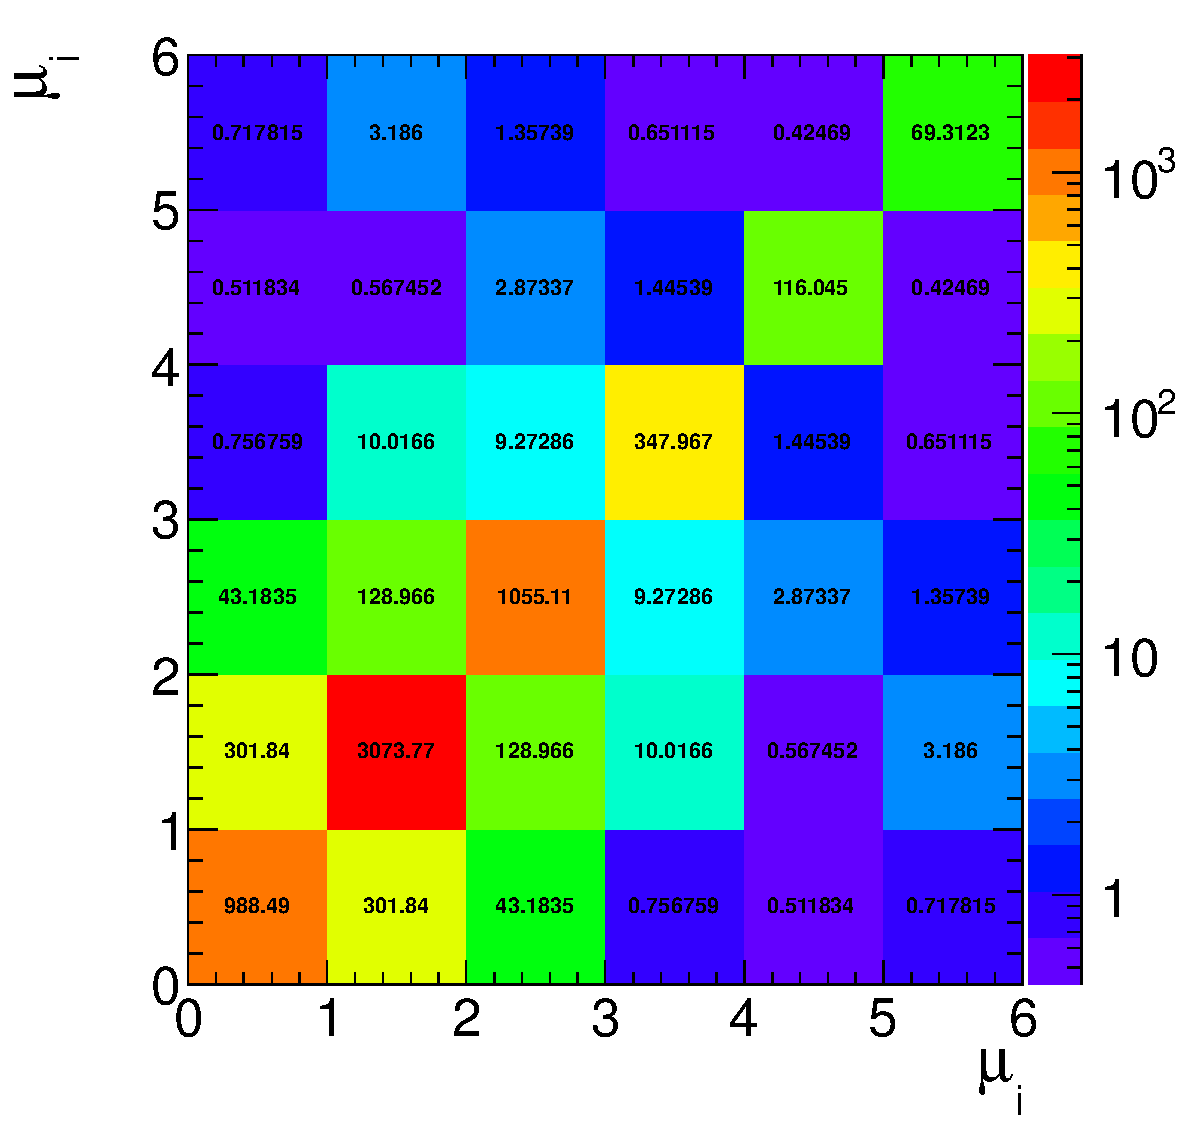
\includegraphics[width=0.6\textwidth]{images/covariance_matrix.pdf}
\caption{Covariance matrix for type A nuisances.\label{fig:covariance_matrix}}
\end{figure}

In the unfolding procedure, errors of type A included in the measured distribution covariance matrix, are propagated to the unfolded distribution.


\subsection{Type B errors}
These errors affect both the signal strength and the response matrix. The nuisances that fall in this category are:
\begin{itemize}
\item the B-veto scale factor (CMS\_8TeV\_btagsf). It affects the signal and background templates by varying the amount of events with jets that enter the selection. It also affects the response matrix because, by varying the fraction of events with jets which are rejected by the veto, it makes the reconstructed spectrum harder or softer.
\item The lepton efficiency scale factor (CMS\_8TeV\_eff\_l). It affects the signal and background template shape and normalization. It affects the response matrix by varying the the reconstructed spectrum.
\item the MET scale and resolution (CMS\_8TeV\_met, CMS\_8TeV\_p\_scale\_met). The effect is similar to above.
\item lepton scale and resolution (CMS\_8TeV\_p\_res\_e, CMS\_8TeV\_p\_scale\_e, CMS\_8TeV\_p\_scale\_m). The effect is similar to above.
\item Jet energy scale (CMS\_8TeV\_p\_scale\_j). It affects the signal and background template shape and normalization. It also affects the response matrix because, by varying the fraction of events with jets, the b veto can reject more or less events, thus making the reconstructed spectrum harder or softer.
\end{itemize}
Since each of these nuisances changes the response matrix in its own way, we cannot extract a global correlation matrix for them, instead we need to evaluate each of them one by one, and then use the varied signal strengths for each of these nuisance in conjunction with the corresponding varied response matrix. In order to evaluate the effect of each of the above mentioned nuisances on the signal strength parameters we have used the following procedure. 
The first step consists in performing a fit letting all nuisance free to float. Then for each type B nuisance we perform two additional fits: one with the nuisance frozen to a + $1~\sigma$ with respect to its nominal value and one freezing the nuisance to -$1~\sigma$ with respect to its nominal value. The difference on the signal strengths between the two variation and the fit with everything floating gives the uncertainty on the signal strengths due to that particular nuisance. This method allows us also to catch the way in which nuisances are correlated across different \pth bins.
%More in details, we calculate the difference between the signal strengths of every bin obtained fitting all the nuisances and the ones obtained freezing a nuisance to its up or down variation. The absolute value of this difference is taken as the upper or lower bound of the error band due to the evaluated nuisance, corresponding to its up or down variation respectively. In case both the up and down variation of a nuisance lead to a deviation of the signal strength in the same direction, only the larger error is taken into account.\\
%As can be observed, the larger effects can be ascribed to the following nuisances: b-tagging (CMS\_8TeV\_btagsf), leptons efficiency (CMS\_8TeV\_eff\_l), MET resolution (CMS\_8TeV\_met) and electron resolution (CMS\_8TeV\_p\_res\_e), MET, leptons and jets scale variations (CMS\_8TeV\_p\_scale\_met, CMS\_8TeV\_p\_scale\_e, CMS\_8TeV\_p\_scale\_m, CMS\_8TeV\_p\_scale\_j). The effect of background normalization uncertainties and on QCD scale variations is smaller, even if not negligible.
The relative errors for each of the type B nuisances is shown in Tab.~\ref{table:corr_syst}. Using these uncertainties, we can build, for each of the type B nuisances, a varied up and a varied down measured spectrum.
%\begin{landscape}
\begin{sidewaystable}
\caption{Effect of all the correlated nuisances on the signal strengths of each bin. In the table are reported the signal strength variations corresponding to an up or down scaling of the nuisance.}\label{table:corr_syst}
\centering
\small{
\begin{tabular}{|c|cccccc|}
\hline
\bf{nuisance} & \bf{bin1} & \bf{bin2} & \bf{bin3} & \bf{bin4} & \bf{bin5} & \bf{bin6} \\ 
\hline 
\hline 
%CMS\_8TeV\_btagsf & -10.0/-8.7 (\%) & 7.5/12.3 (\%) & -7.1/2.2 (\%) & -9.2/2.2 (\%) & -4.1/13.8 (\%) & -8.2/18.1 (\%) \\ 
%CMS\_8TeV\_eff\_l & -14.6/-3.7 (\%) & 4.6/15.2 (\%) & -6.5/1.7 (\%) & -7.6/0.8 (\%) & 0.4/8.1 (\%) & -0.2/6.6 (\%) \\  
%CMS\_8TeV\_met & -14.5/0.0 (\%) & 13.7/-0.0 (\%) & -11.3/-0.0 (\%) & 3.9/0.0 (\%) & -28.2/-0.0 (\%) & 15.8/0.0 (\%) \\  
%CMS\_8TeV\_p\_res\_e & -12.4/-0.0 (\%) & 11.2/0.0 (\%) & -3.8/0.0 (\%) & -6.5/-0.0 (\%) & 11.8/0.0 (\%) & -6.3/-0.0 (\%) \\ 
%CMS\_8TeV\_p\_scale\_e & -2.9/-15.6 (\%) & 15.7/7.8 (\%) & 10.3/-17.0 (\%) & 20.3/-27.1 (\%) & 32.7/-12.4 (\%) & 11.5/-10.8 (\%) \\ 
%CMS\_8TeV\_p\_scale\_j & -10.7/-9.9 (\%) & 9.2/9.1 (\%) & -3.9/-3.8 (\%) & -4.3/-3.2 (\%) & 1.2/4.0 (\%) & 4.8/2.9 (\%) \\  
%CMS\_8TeV\_p\_scale\_m & -6.7/-11.4 (\%) & 11.9/8.4 (\%) & -0.0/-9.5 (\%) & 6.1/-8.8 (\%) & 13.7/-2.6 (\%) & 8.2/-1.6 (\%) \\ 
%CMS\_8TeV\_p\_scale\_met & -14.1/-9.9 (\%) & 0.2/15.4 (\%) & -3.7/-6.5 (\%) & 2.3/-20.2 (\%) & -1.3/27.5 (\%) & 3.0/7.6 (\%) \\
CMS\_8TeV\_btagsf & -10.1/-8.8 (\%) & 7.3/12.2 (\%) & -6.3/3.1 (\%) & -14.4/-4.8 (\%) & -5.4/14.5 (\%) & -7.9/17.8 (\%) \\ 
CMS\_8TeV\_eff\_l & -14.7/-3.9 (\%) & 4.5/15.1 (\%) & -5.7/2.5 (\%) & -13.2/-5.3 (\%) & -0.2/7.6 (\%) & -0.1/6.8 (\%) \\ 
CMS\_8TeV\_met & -12.5/0.0 (\%) & 15.4/-0.0 (\%) & -12.8/-0.0 (\%) & 8.7/0.0 (\%) & -20.9/-0.0 (\%) & 10.5/0.0 (\%) \\ 
CMS\_8TeV\_p\_res\_e & -12.5/-0.0 (\%) & 11.2/0.0 (\%) & -2.4/0.0 (\%) & -13.4/-0.0 (\%) & 9.9/0.0 (\%) & -4.6/-0.0 (\%) \\ 
CMS\_8TeV\_p\_scale\_e & -2.7/-13.1 (\%) & 15.9/9.9 (\%) & 10.8/-16.8 (\%) & 16.2/-33.1 (\%) & 30.9/-14.4 (\%) & 12.6/-10.9 (\%) \\ 
CMS\_8TeV\_p\_scale\_j & -10.9/-10.1 (\%) & 9.0/9.0 (\%) & -3.0/-2.9 (\%) & -10.3/-8.9 (\%) & 0.3/3.4 (\%) & 5.2/3.1 (\%) \\
CMS\_8TeV\_p\_scale\_m & -7.0/-10.7 (\%) & 11.8/8.9 (\%) & 1.1/-8.7 (\%) & -0.7/-14.4 (\%) & 14.5/-4.6 (\%) & 8.0/-1.6 (\%) \\ 
CMS\_8TeV\_p\_scale\_met & -14.4/-6.8 (\%) & -0.0/17.7 (\%) & -6.1/-7.1 (\%) & 9.6/-20.9 (\%) & 2.3/32.4 (\%) & 2.5/2.6 (\%) \\ 

\hline
\end{tabular}
}
\end{sidewaystable}
%\end{landscape}

For each of the type B nuisances we also build an up and a down varied response matrix.
For each type B nuisance we can thus build an unfolded varied up and varied down spectrum, simply by applying the unfolding to the varied spectrum using the corresponding varied response matrix.


\subsubsection{Likelihood scans}\label{subsec:bananas}
In order to further validate the numbers reported in the table \ref{table:corr_syst} and to verify the goodness of the fitting procedure, a scan of the likelihood function has been performed using a grid of points in a two-dimensional space. \\
In the following, a nuisance value of 0 corresponds to its nominal value while the $\pm 1 \sigma$ variations correspond exactly to $\pm 1$ values.\\
The scan has been performed in the nuisance/signal strength space for some correlated nuisances and for all the $p_T^H$ bins, taking the nuisance and the signal strength as parameters of interest. For each parameters of interest/nuisance pair a 10000 points grid scan of the likelihood function is performed. In this way a two-dimensional likelihood scan is obtained. To verify the numbers in table \ref{table:corr_syst} the two-dimensional likelihood plot has been divided in several slices and the one-dimensional likelihood slice corresponding to the upper and lower variation of the nuisance, i.e. $nuisance=1$ or $nuisance=-1$ respectively, are shown as a function of the signal strength of a given bin.\\ In this way we can determine if the likelihood function has a reasonable trend and if the minimum corresponds to the value shown in the table.\\
In figures \ref{fig:btagsf_bananas_p1} and \ref{fig:btagsf_bananas_p2} are reported the two-dimensional scans and the corresponding $\pm 1 \sigma$ profiles for the b-tagging nuisance in each $p_T^H$ bin. The scans have been performed varying the nuisance in the range from $-2$ to $+2$ and the signal strengths from $0$ to $+2$.
 All the scans show the expected trend and the minimum points of the profiles, pointed out by dashed vertical lines, correspond to the numbers in the correlated systematics table.\\
 In figures \ref{fig:eff_l_bananas_p1} and \ref{fig:eff_l_bananas_p2} are shown the same plots but, in this case, scanning the lepton efficiency nuisance.

\begin{figure}[htb]
\centering
\subfigure[CMS\_8TeV\_btagsf vs $\mu_0$]{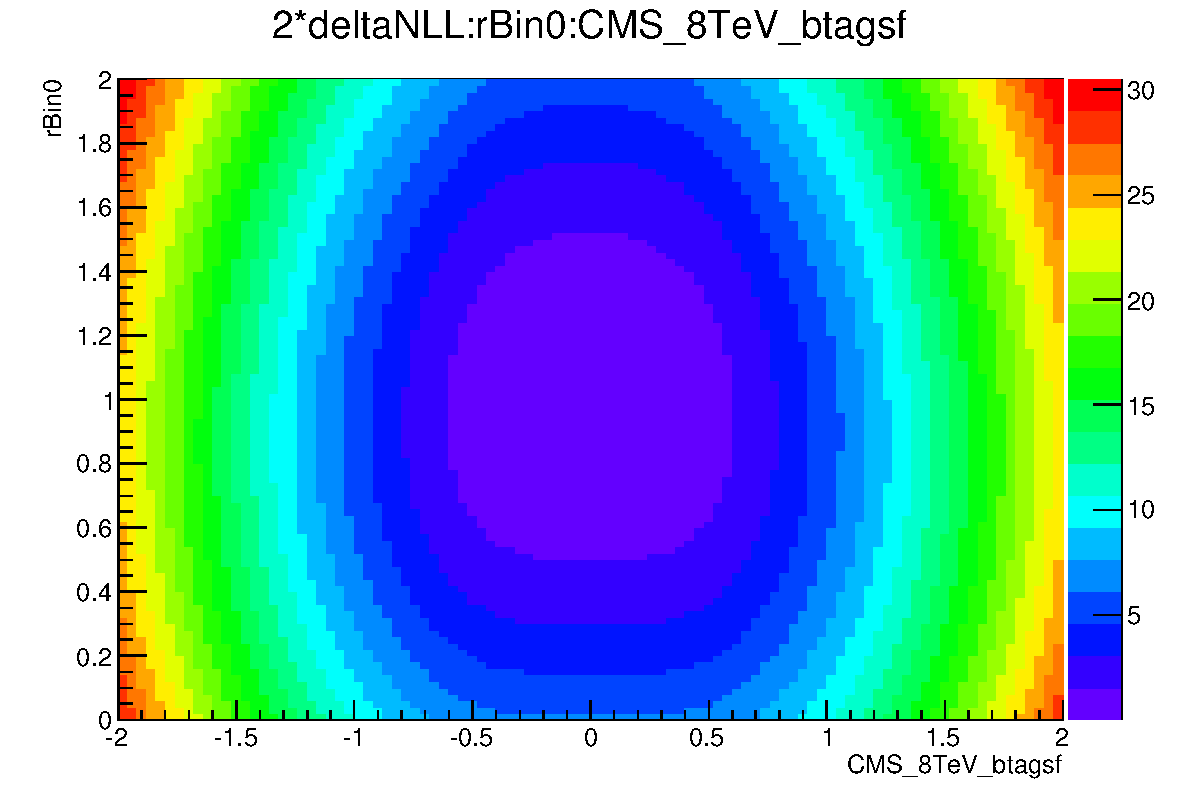
\includegraphics[width=0.45\textwidth]{images/bananas/rBin0_CMS_8TeV_btagsf.pdf}}
\subfigure[$\mu_0$ profiles]{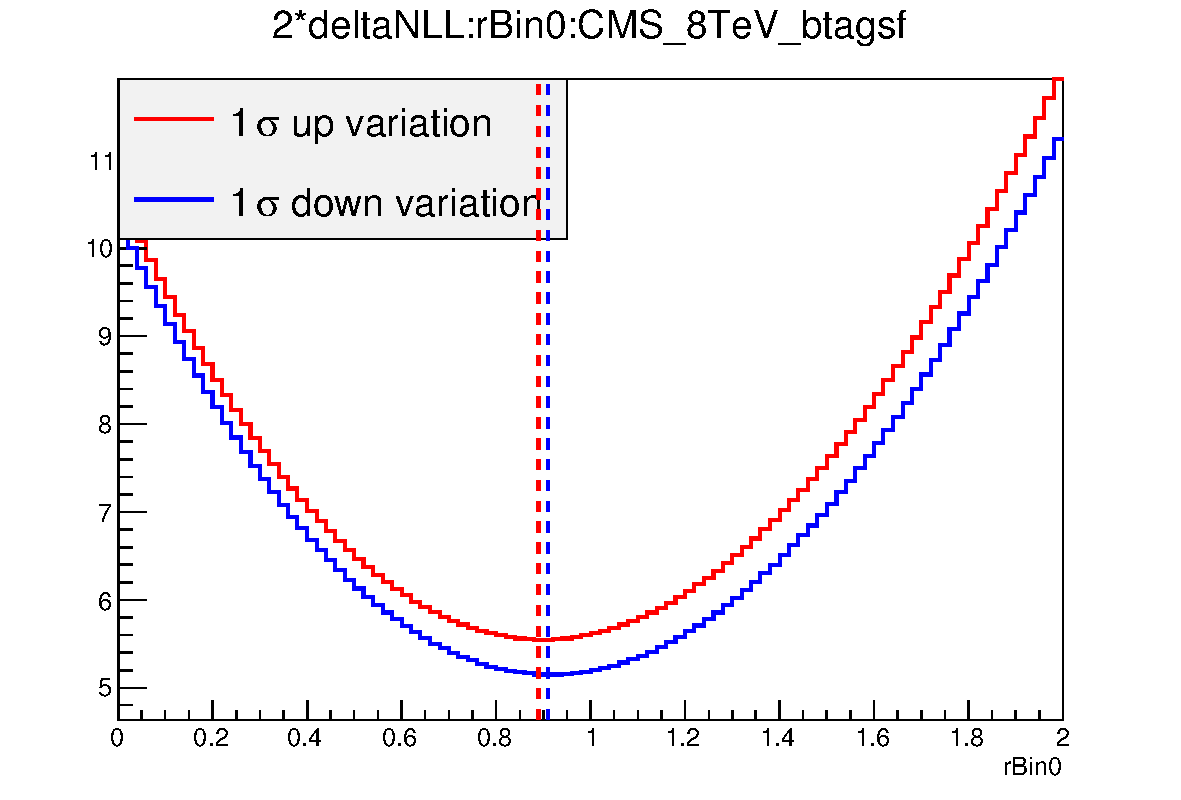
\includegraphics[width=0.45\textwidth]{images/bananas/profile_rBin0_CMS_8TeV_btagsf.pdf}}\\

\subfigure[CMS\_8TeV\_btagsf vs $\mu_1$]{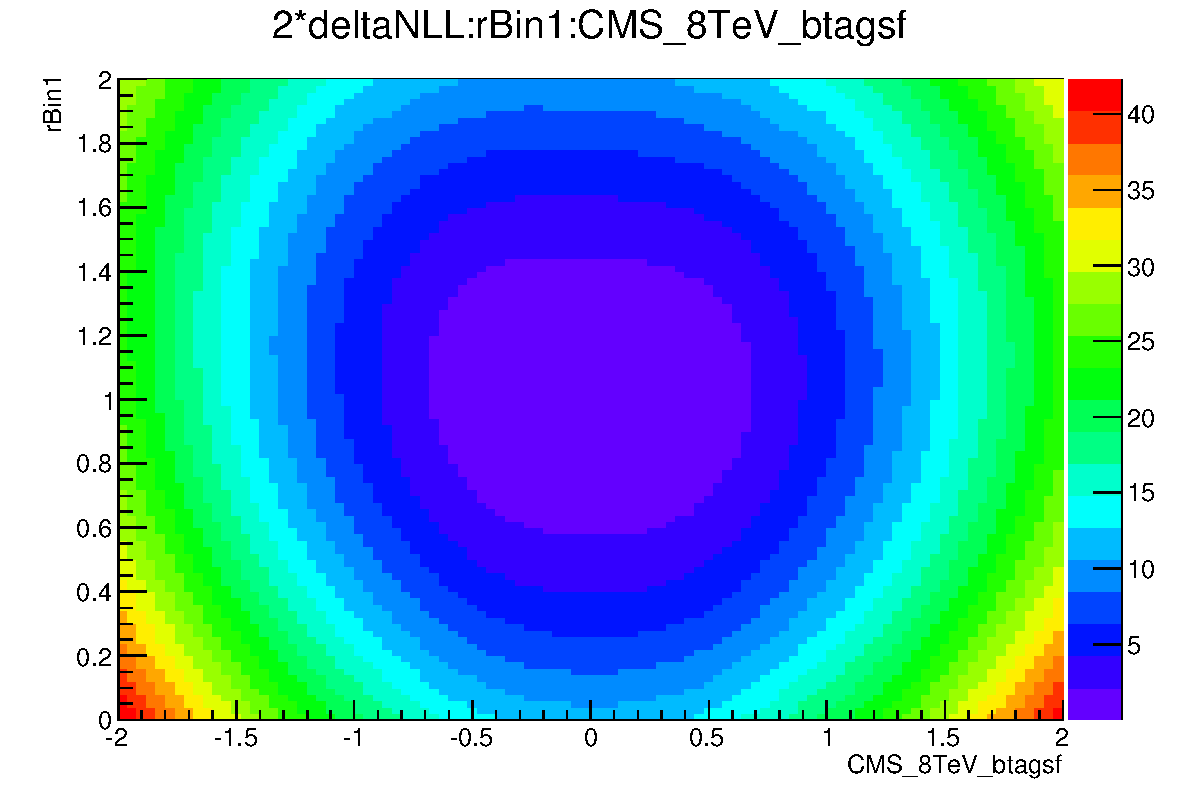
\includegraphics[width=0.45\textwidth]{images/bananas/rBin1_CMS_8TeV_btagsf.pdf}}
\subfigure[$\mu_1$ profiles]{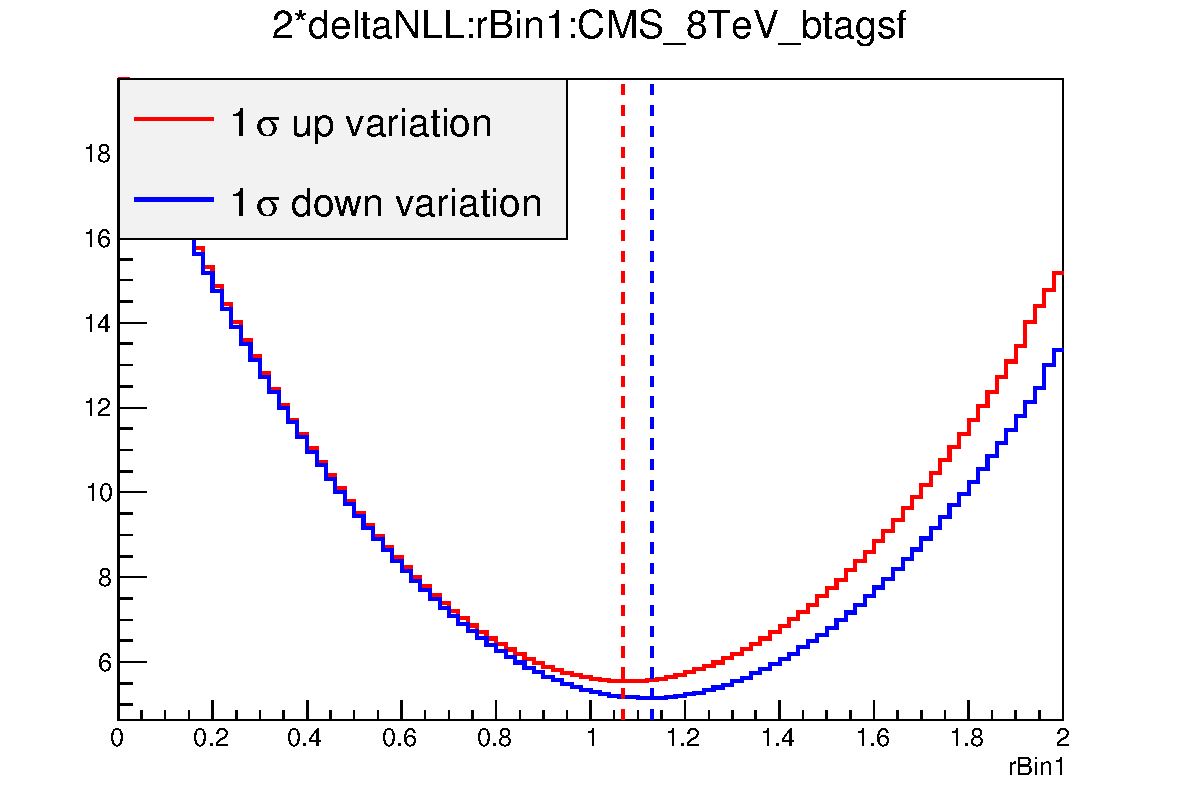
\includegraphics[width=0.45\textwidth]{images/bananas/profile_rBin1_CMS_8TeV_btagsf.pdf}}\\

\subfigure[CMS\_8TeV\_btagsf vs $\mu_2$]{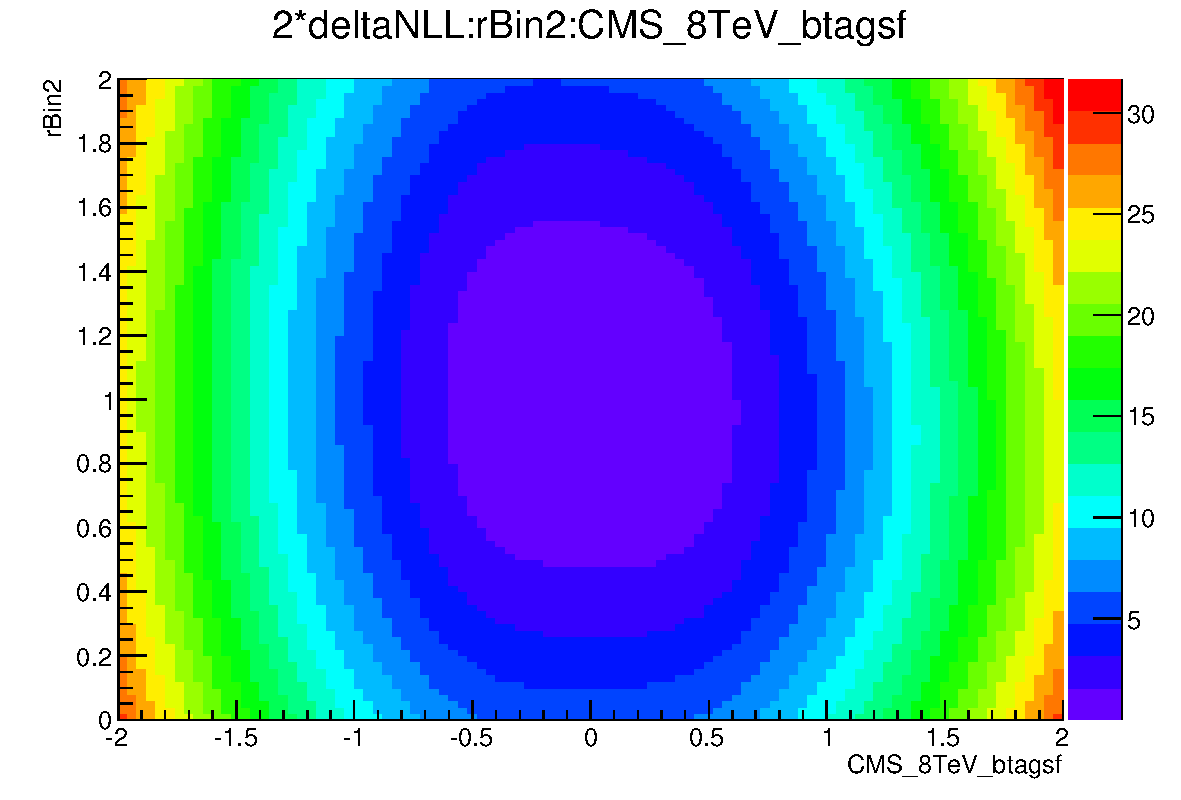
\includegraphics[width=0.45\textwidth]{images/bananas/rBin2_CMS_8TeV_btagsf.pdf}}
\subfigure[$\mu_2$ profiles]{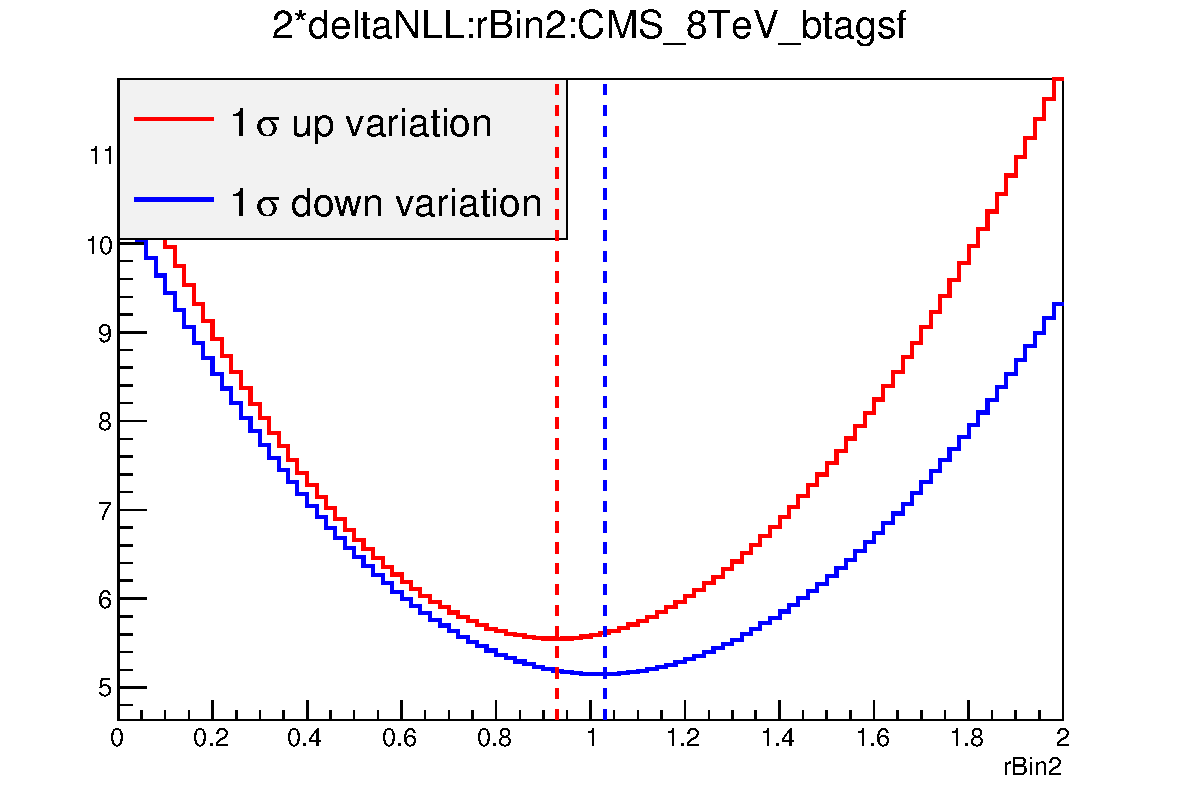
\includegraphics[width=0.45\textwidth]{images/bananas/profile_rBin2_CMS_8TeV_btagsf.pdf}}\\

\caption{{\bf Left side} Two-dimensional likelihood scan for b-tagging nuisance vs signal strengths in several bins: (a) bin 0, (c) bin 1, (e) bin 2. {\bf Right side} Likelihood profiles corresponding to the nuisance $\pm 1 \sigma$ up/down variations for (b) bin 0, (d) bin 1 and (f) bin 2. \label{fig:btagsf_bananas_p1}}
\end{figure}

\begin{figure}[htb]
\centering

\subfigure[CMS\_8TeV\_btagsf vs $\mu_3$]{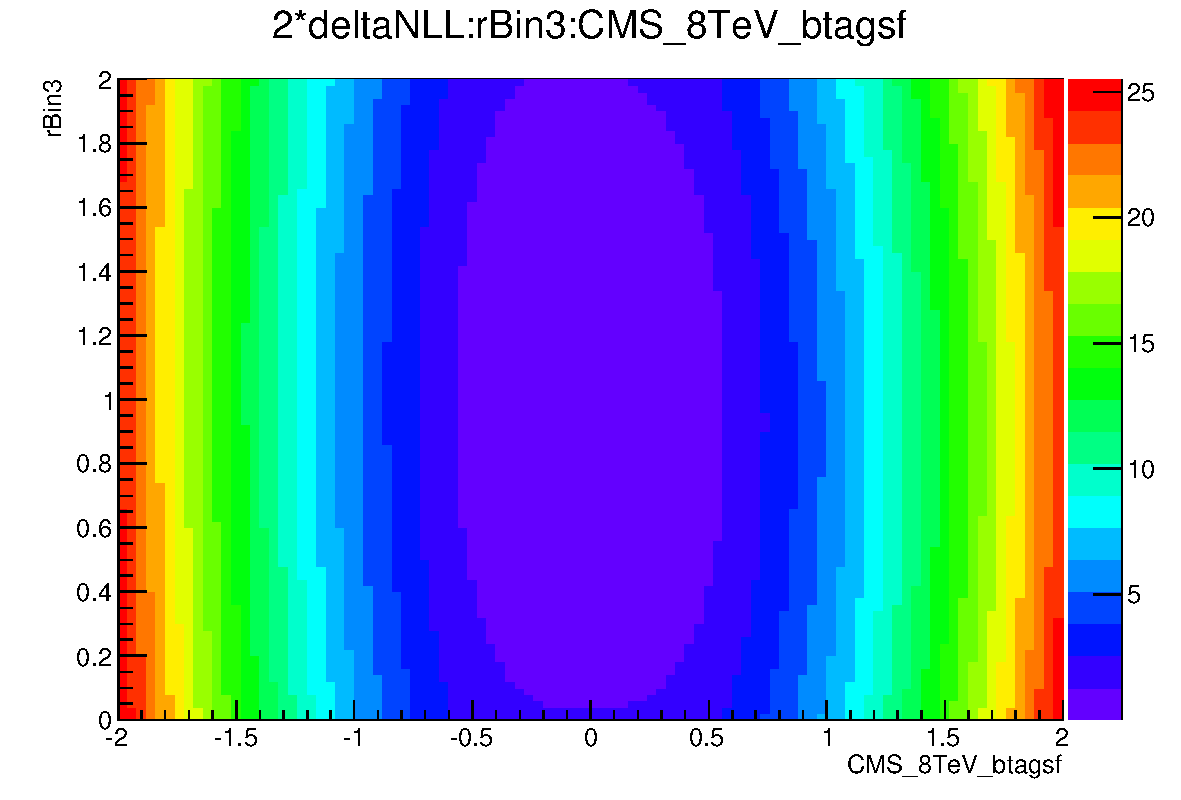
\includegraphics[width=0.45\textwidth]{images/bananas/rBin3_CMS_8TeV_btagsf.pdf}}
\subfigure[$\mu_3$ profiles]{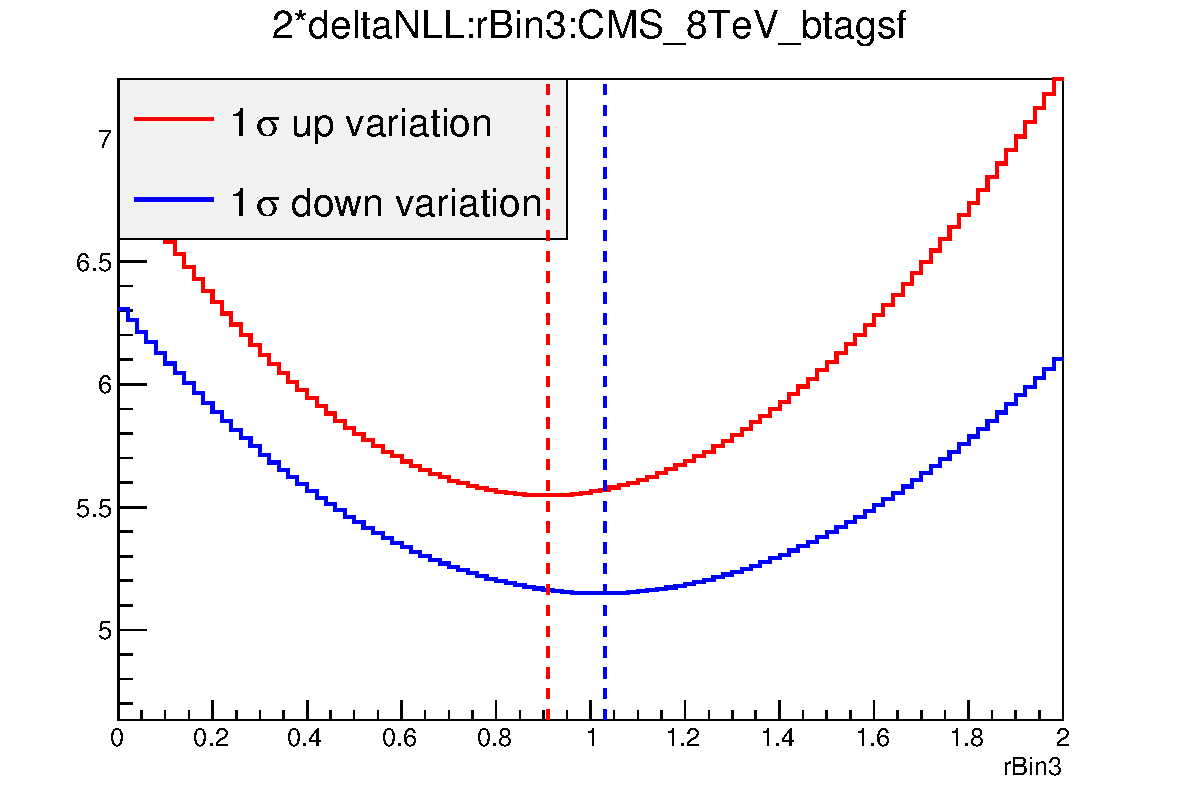
\includegraphics[width=0.45\textwidth]{images/bananas/profile_rBin3_CMS_8TeV_btagsf.pdf}}

\subfigure[CMS\_8TeV\_btagsf vs $\mu_4$]{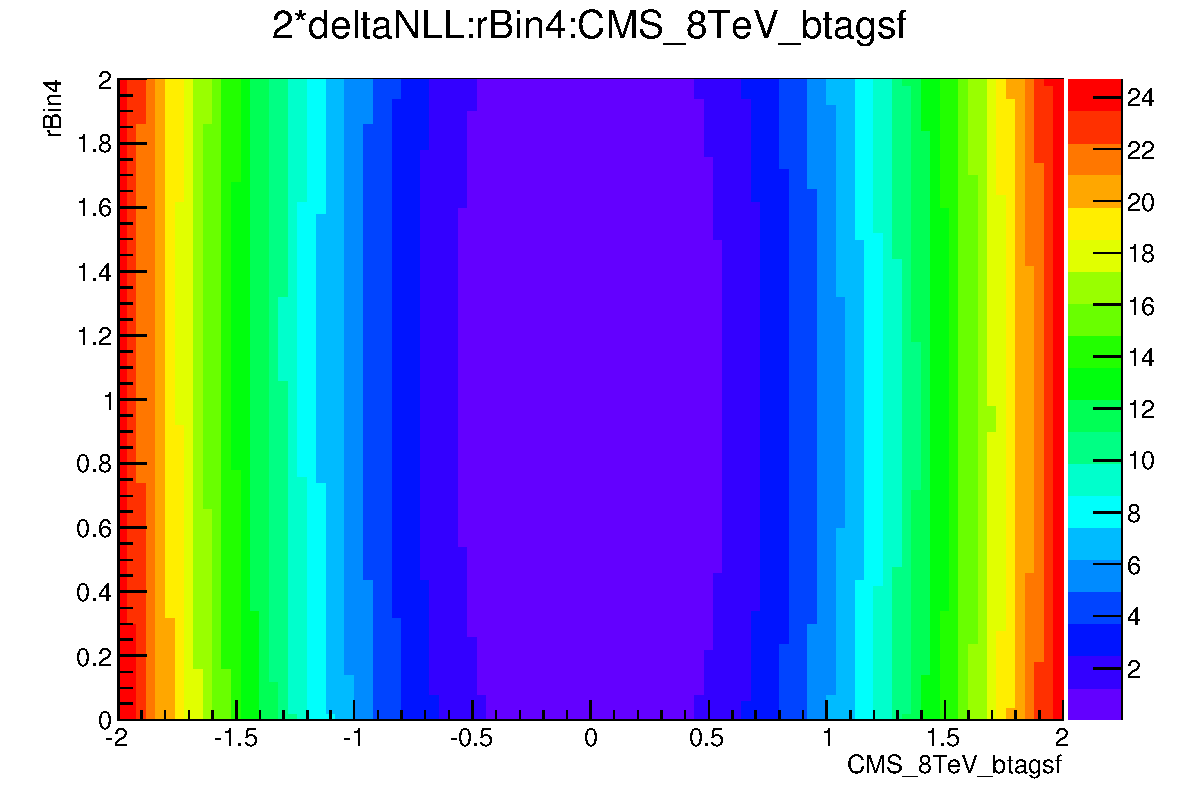
\includegraphics[width=0.45\textwidth]{images/bananas/rBin4_CMS_8TeV_btagsf.pdf}}
\subfigure[$\mu_4$ profiles]{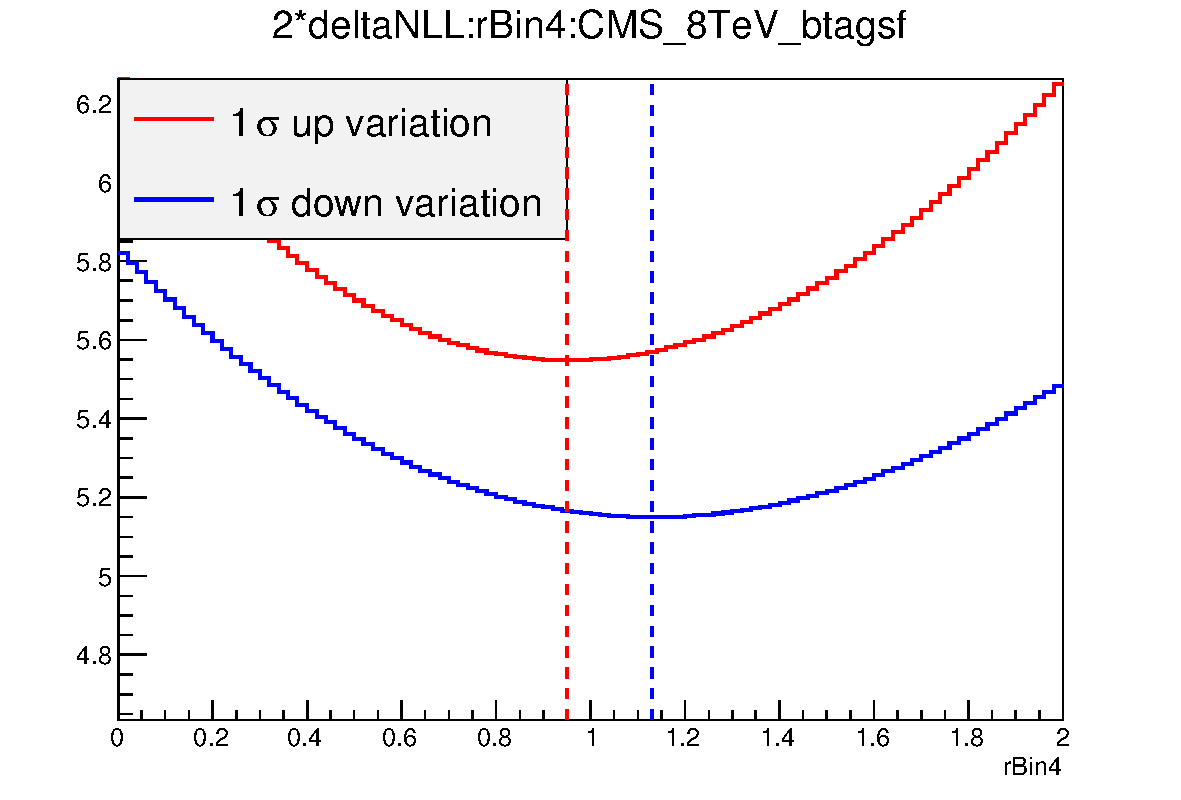
\includegraphics[width=0.45\textwidth]{images/bananas/profile_rBin4_CMS_8TeV_btagsf.pdf}}\\

\subfigure[CMS\_8TeV\_btagsf vs $\mu_5$]{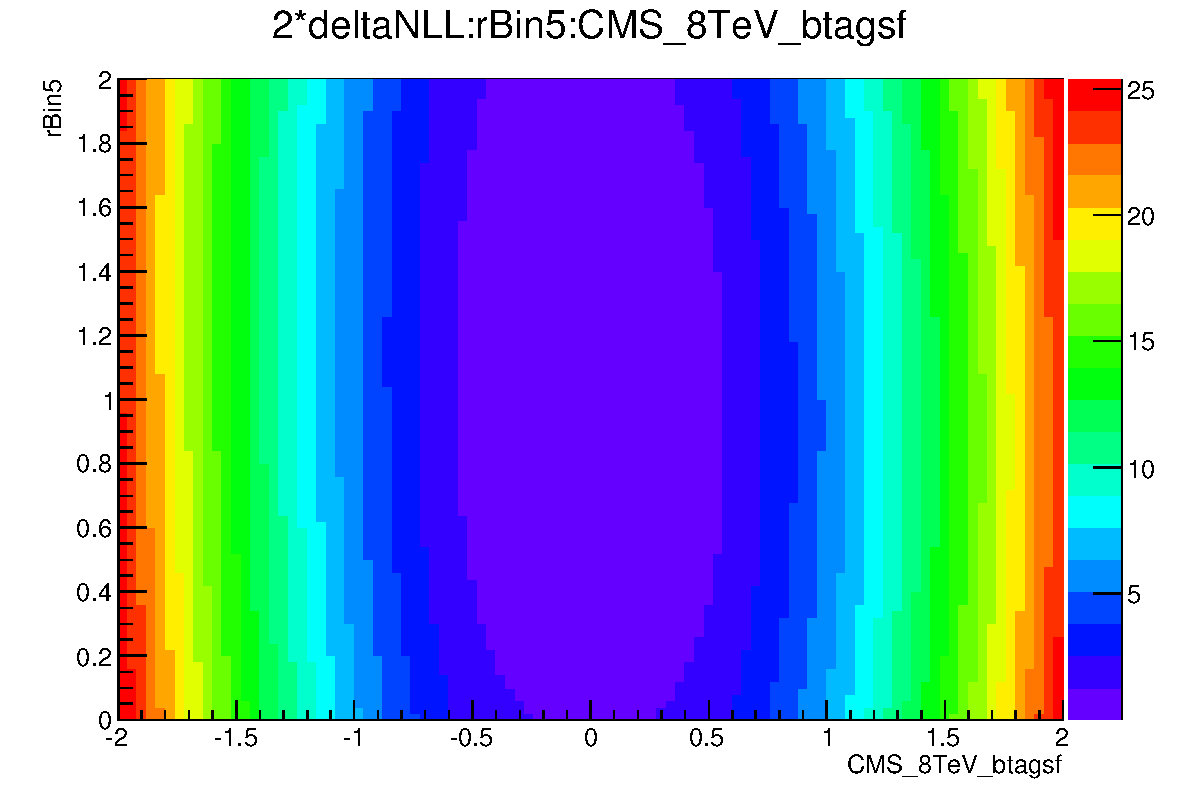
\includegraphics[width=0.45\textwidth]{images/bananas/rBin5_CMS_8TeV_btagsf.pdf}}
\subfigure[$\mu_5$ profiles]{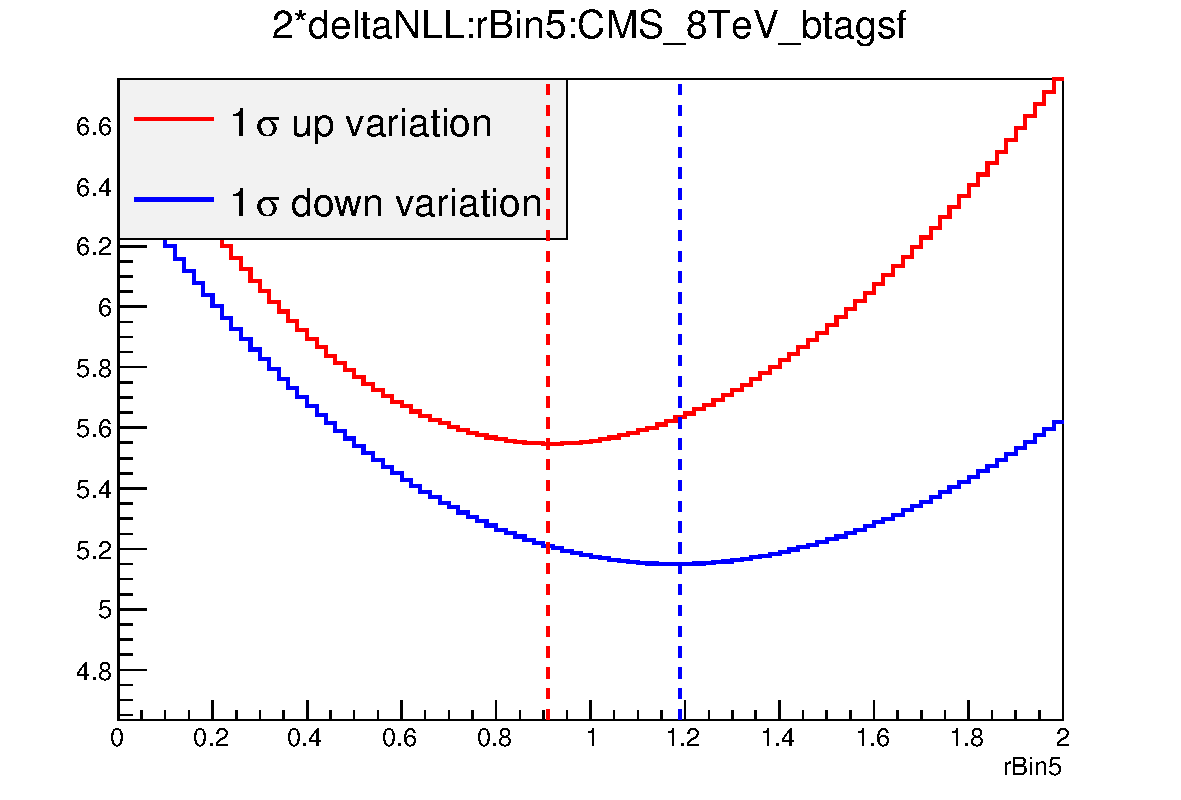
\includegraphics[width=0.45\textwidth]{images/bananas/profile_rBin5_CMS_8TeV_btagsf.pdf}}\\

\caption{{\bf Left side} Two-dimensional likelihood scan for b-tagging nuisance vs signal strengths in several bins: (a) bin 3, (c) bin 4, (e) bin 5. {\bf Right side} Likelihood profiles corresponding to the nuisance $\pm 1 \sigma$ up/down variations for (b) bin 3, (d) bin 4 and (f) bin 5.\label{fig:btagsf_bananas_p2}}
\end{figure}



\begin{figure}[htb]
\centering
\subfigure[CMS\_8TeV\_eff\_l vs $\mu_0$]{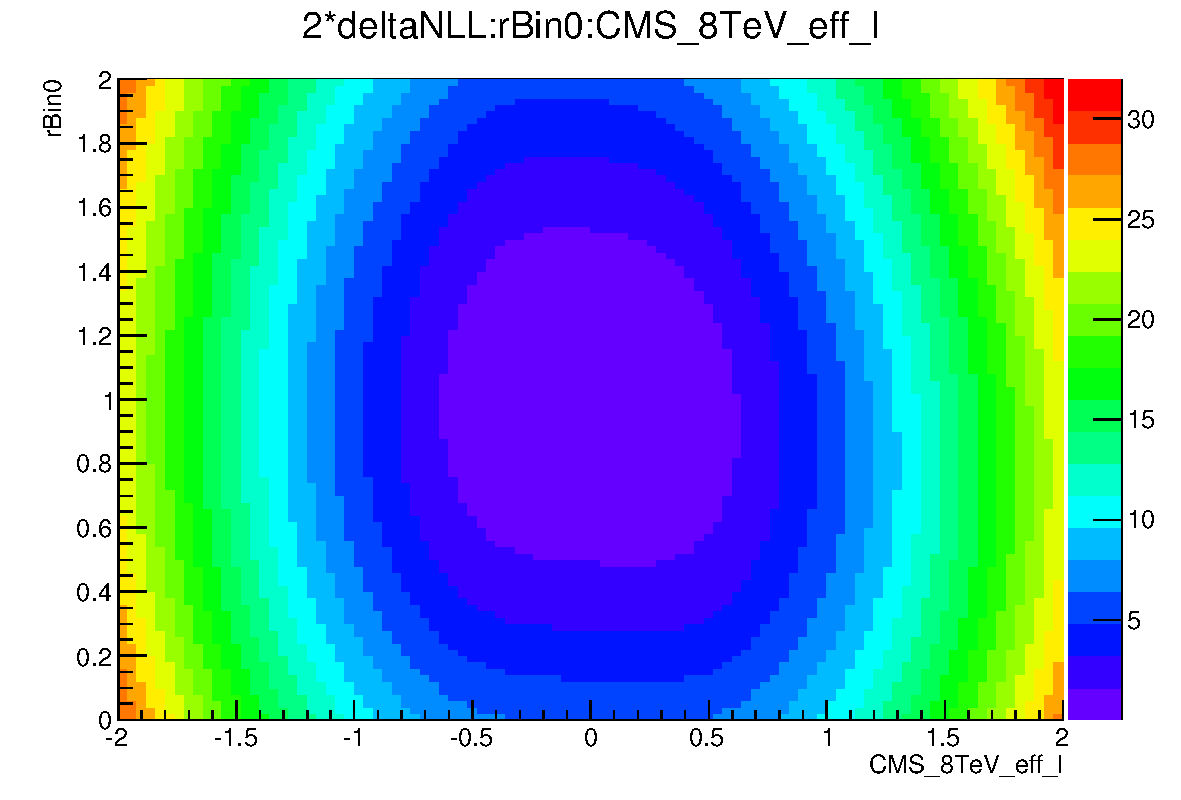
\includegraphics[width=0.45\textwidth]{images/bananas/rBin0_CMS_8TeV_eff_l.pdf}}
\subfigure[$\mu_0$ profiles]{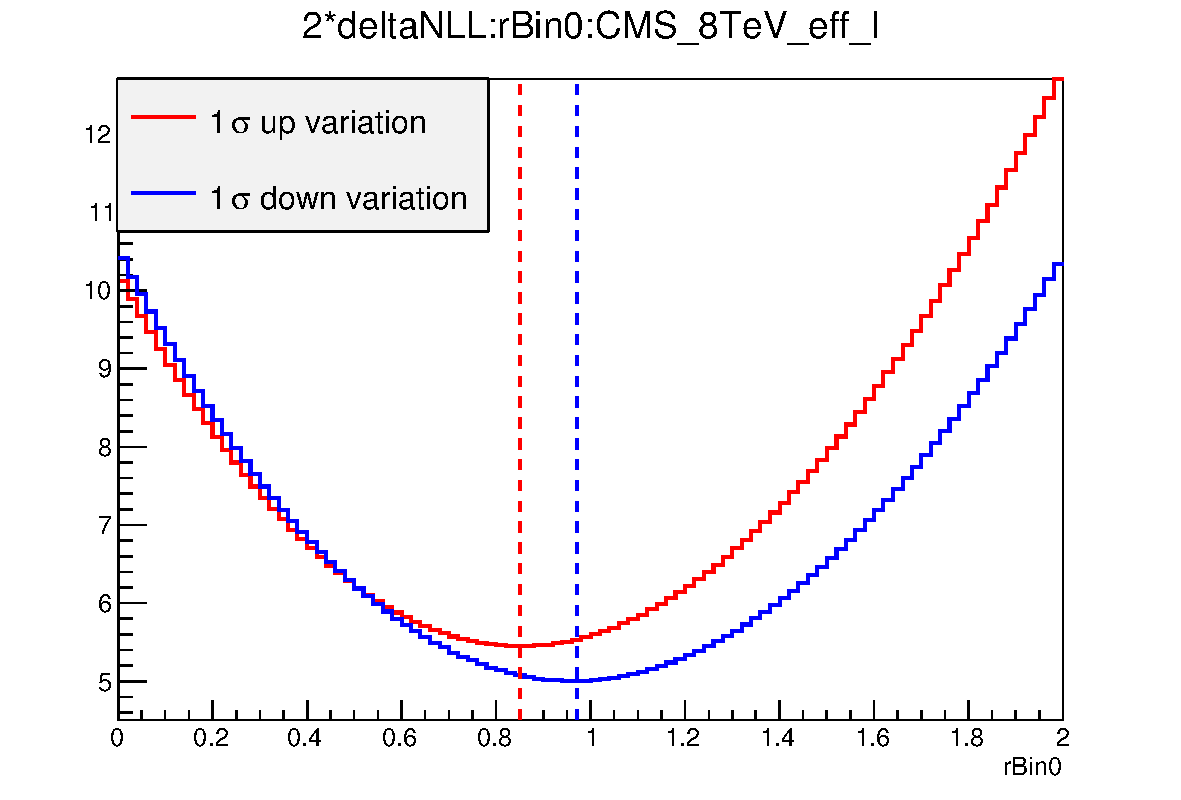
\includegraphics[width=0.45\textwidth]{images/bananas/profile_rBin0_CMS_8TeV_eff_l.pdf}}\\

\subfigure[CMS\_8TeV\_eff\_l vs $\mu_1$]{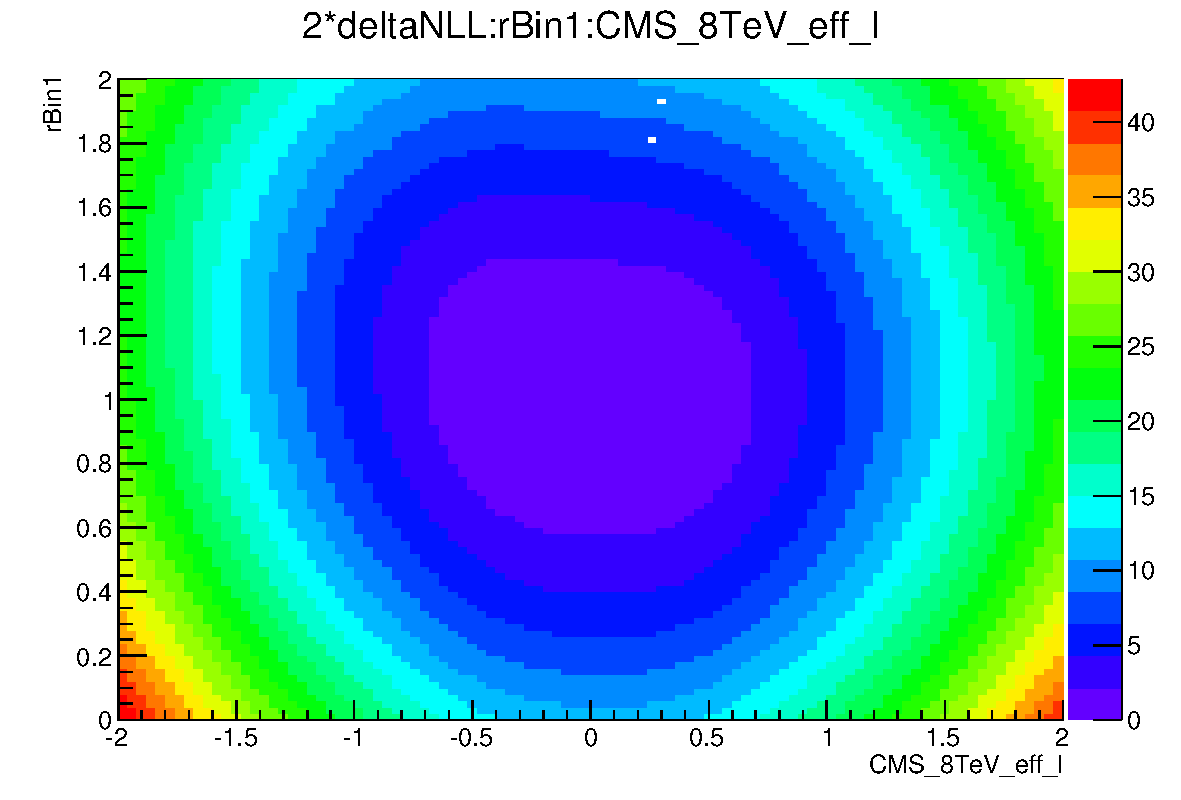
\includegraphics[width=0.45\textwidth]{images/bananas/rBin1_CMS_8TeV_eff_l.pdf}}
\subfigure[$\mu_1$ profiles]{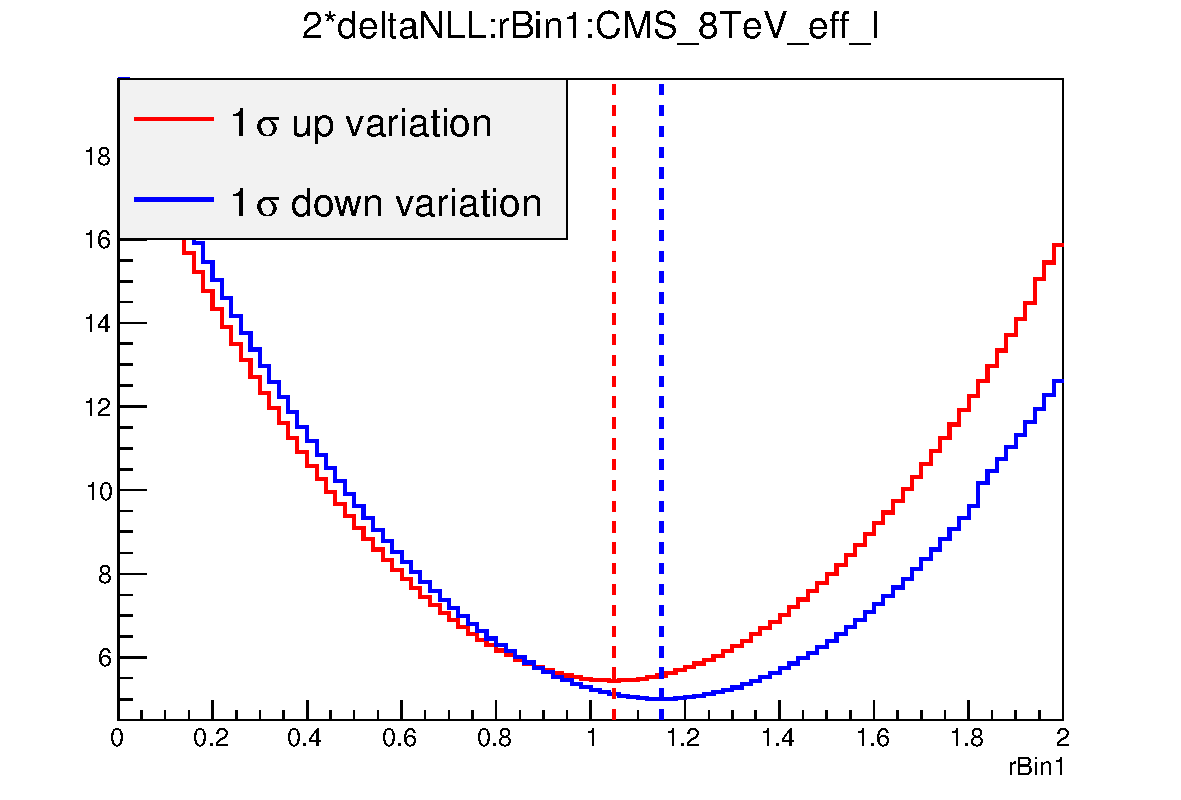
\includegraphics[width=0.45\textwidth]{images/bananas/profile_rBin1_CMS_8TeV_eff_l.pdf}}\\

\subfigure[CMS\_8TeV\_eff\_l vs $\mu_2$]{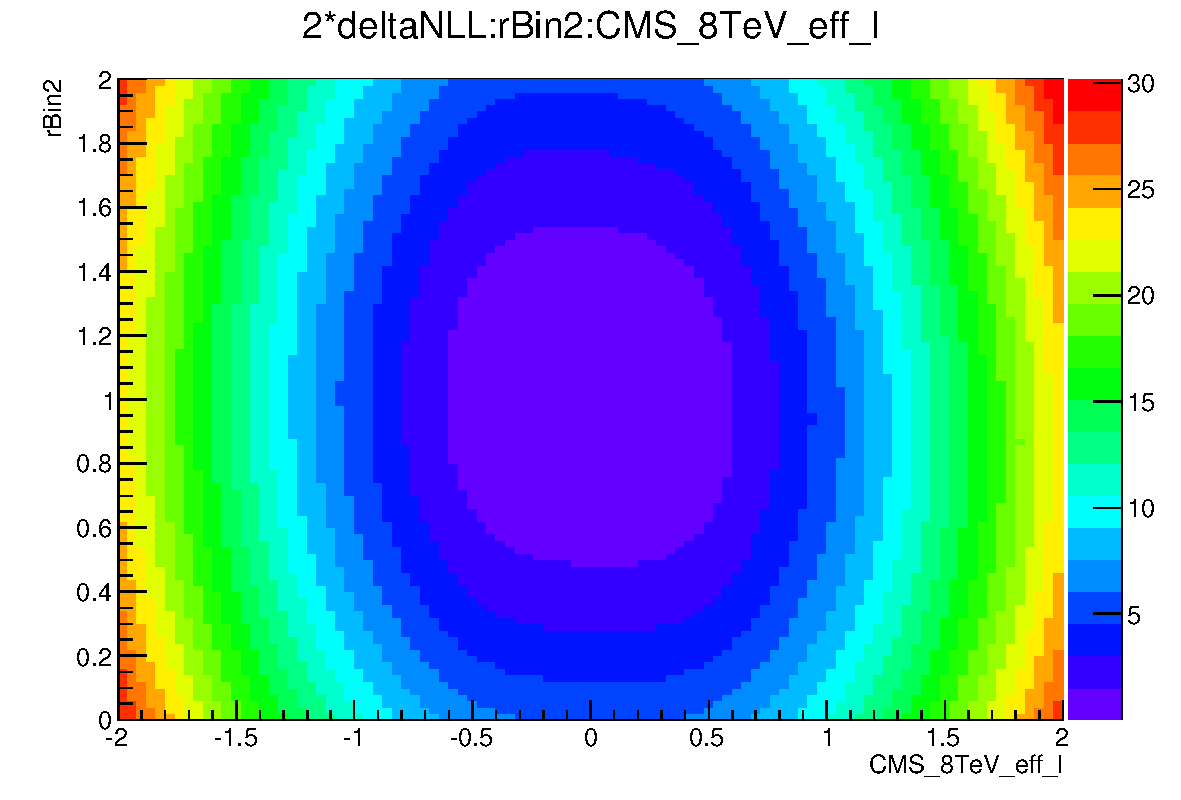
\includegraphics[width=0.45\textwidth]{images/bananas/rBin2_CMS_8TeV_eff_l.pdf}}
\subfigure[$\mu_2$ profiles]{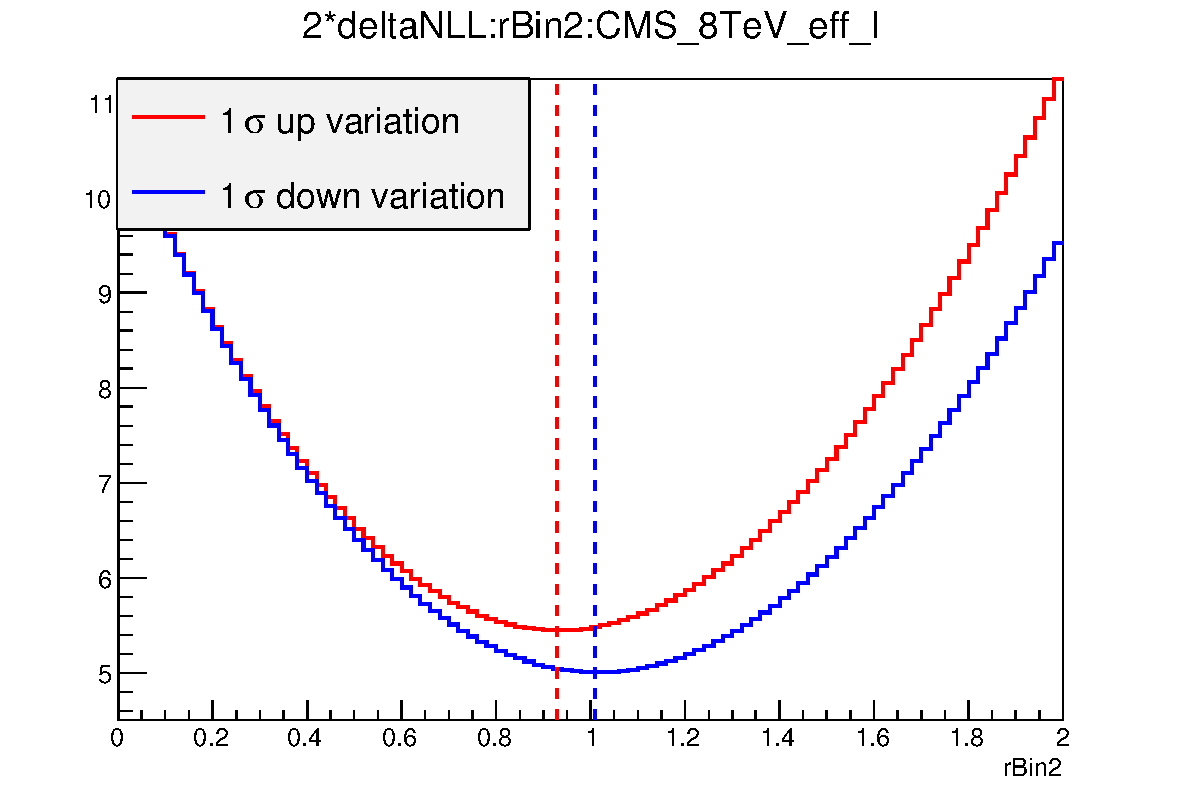
\includegraphics[width=0.45\textwidth]{images/bananas/profile_rBin2_CMS_8TeV_eff_l.pdf}}\\

\caption{{\bf Left side} Two-dimensional likelihood scan for lepton efficiency nuisance vs signal strengths in several bins: (a) bin 0, (c) bin 1, (e) bin 2. {\bf Right side} Likelihood profiles corresponding to the nuisance $\pm 1 \sigma$ up/down variations for (b) bin 0, (d) bin 1 and (f) bin 2.\label{fig:eff_l_bananas_p1}}
\end{figure}


\begin{figure}[htb]
\centering

\subfigure[CMS\_8TeV\_eff\_l vs $\mu_3$]{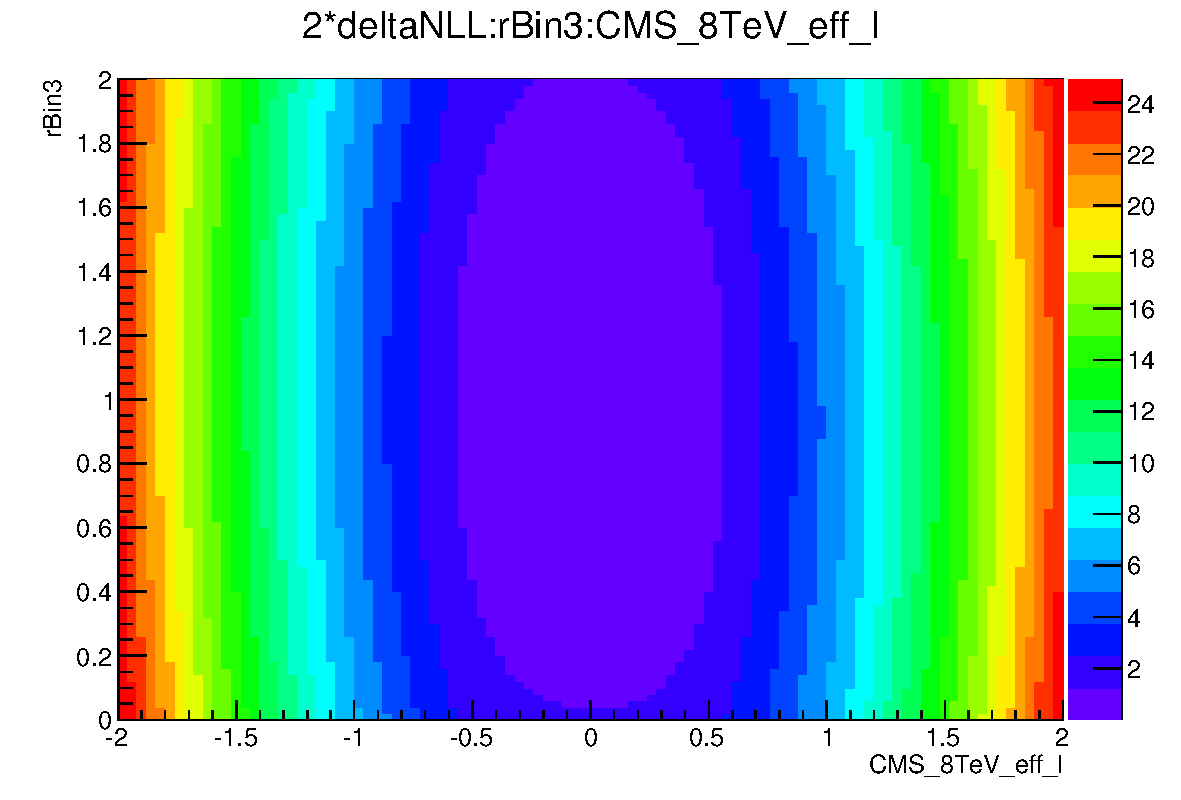
\includegraphics[width=0.45\textwidth]{images/bananas/rBin3_CMS_8TeV_eff_l.pdf}}
\subfigure[$\mu_3$ profiles]{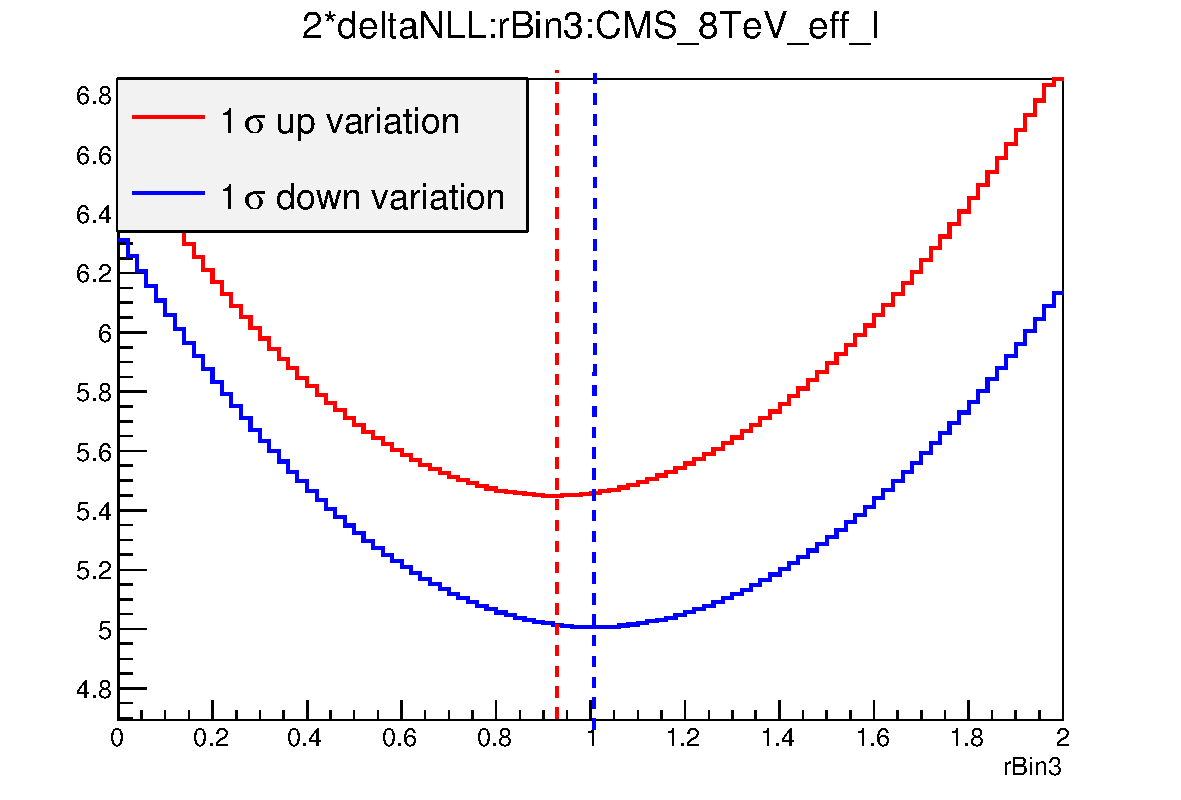
\includegraphics[width=0.45\textwidth]{images/bananas/profile_rBin3_CMS_8TeV_eff_l.pdf}}

\subfigure[CMS\_8TeV\_eff\_l vs $\mu_4$]{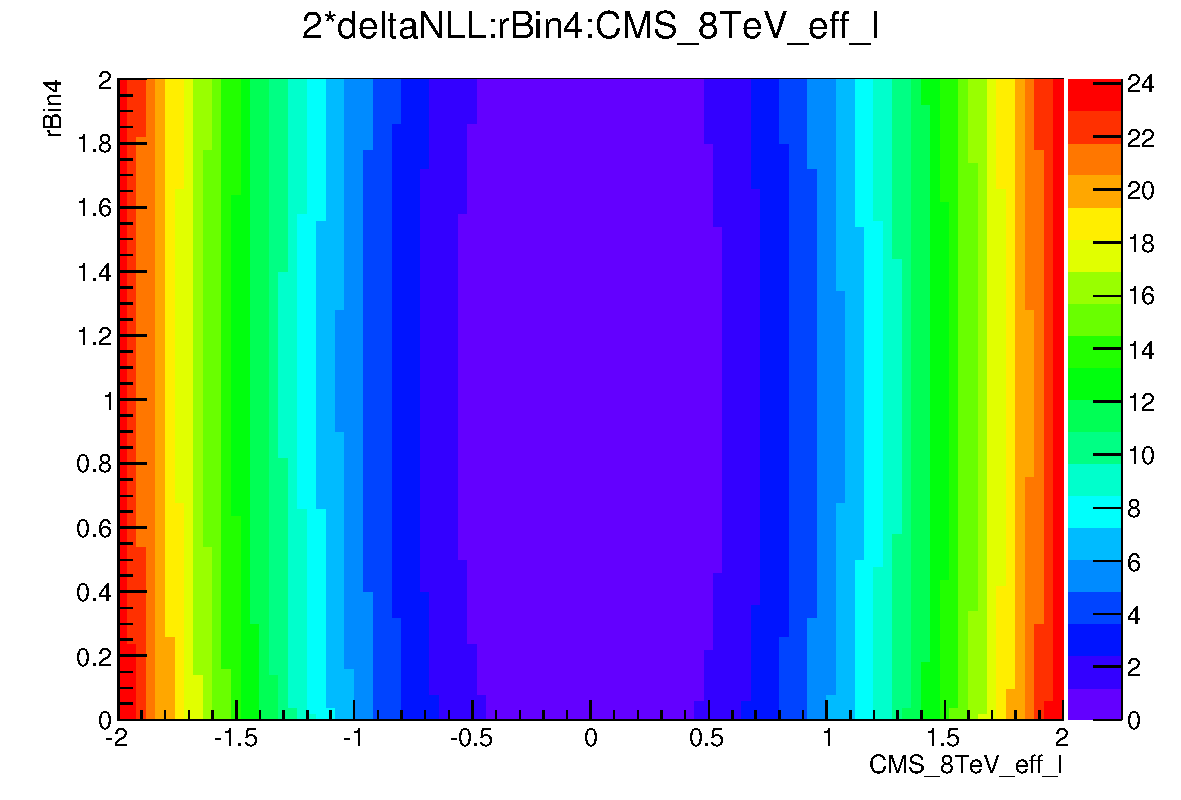
\includegraphics[width=0.45\textwidth]{images/bananas/rBin4_CMS_8TeV_eff_l.pdf}}
\subfigure[$\mu_4$ profiles]{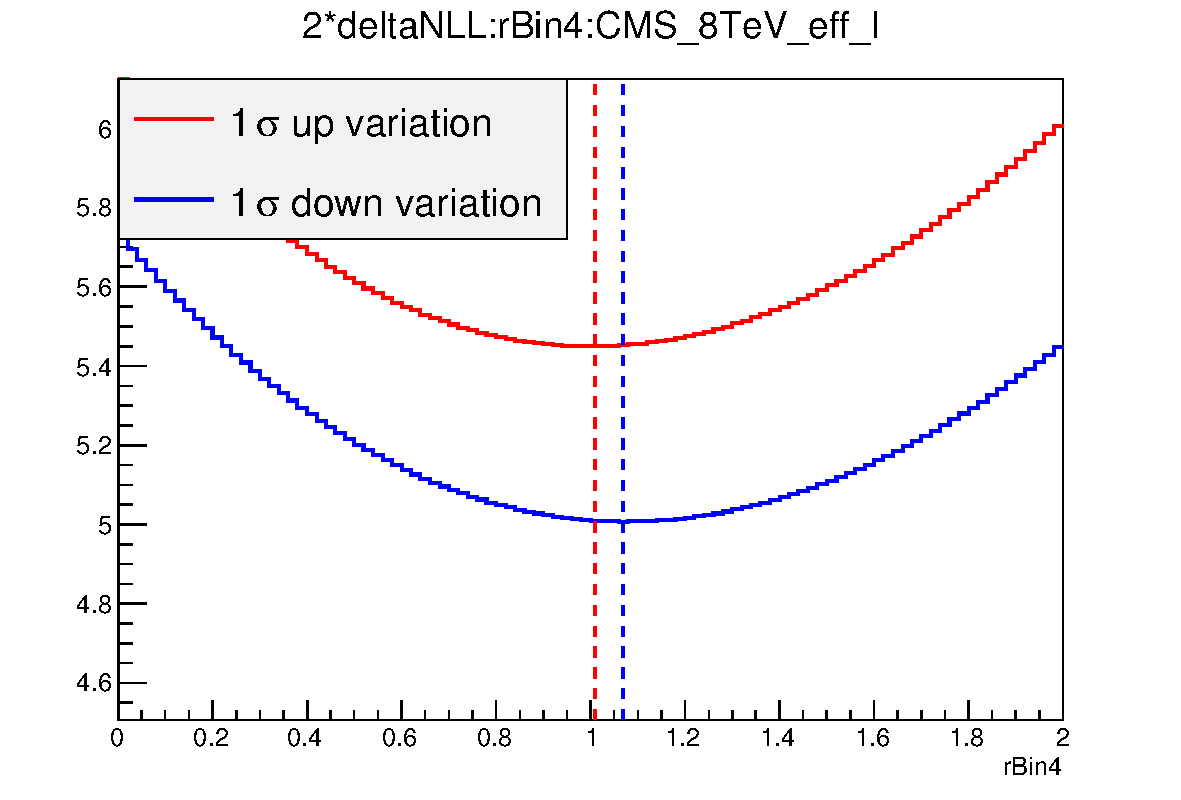
\includegraphics[width=0.45\textwidth]{images/bananas/profile_rBin4_CMS_8TeV_eff_l.pdf}}\\

\subfigure[CMS\_8TeV\_eff\_l vs $\mu_5$]{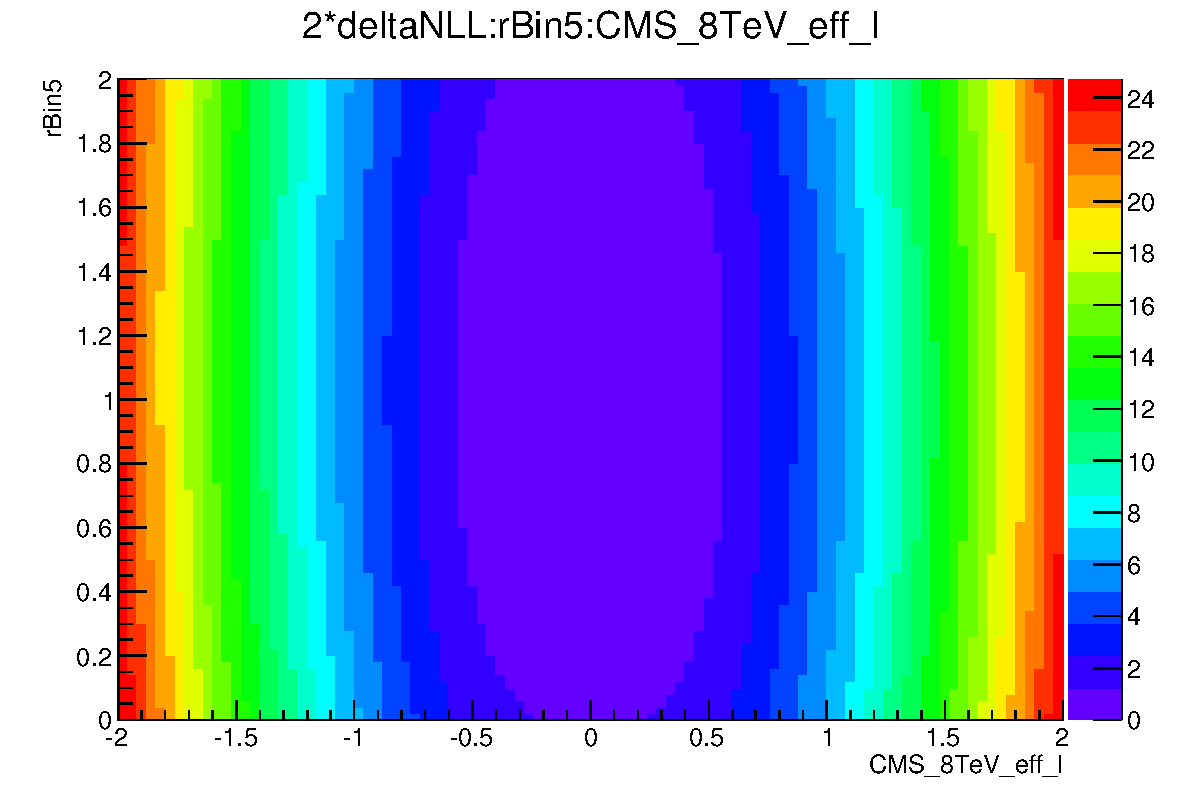
\includegraphics[width=0.45\textwidth]{images/bananas/rBin5_CMS_8TeV_eff_l.pdf}}
\subfigure[$\mu_5$ profiles]{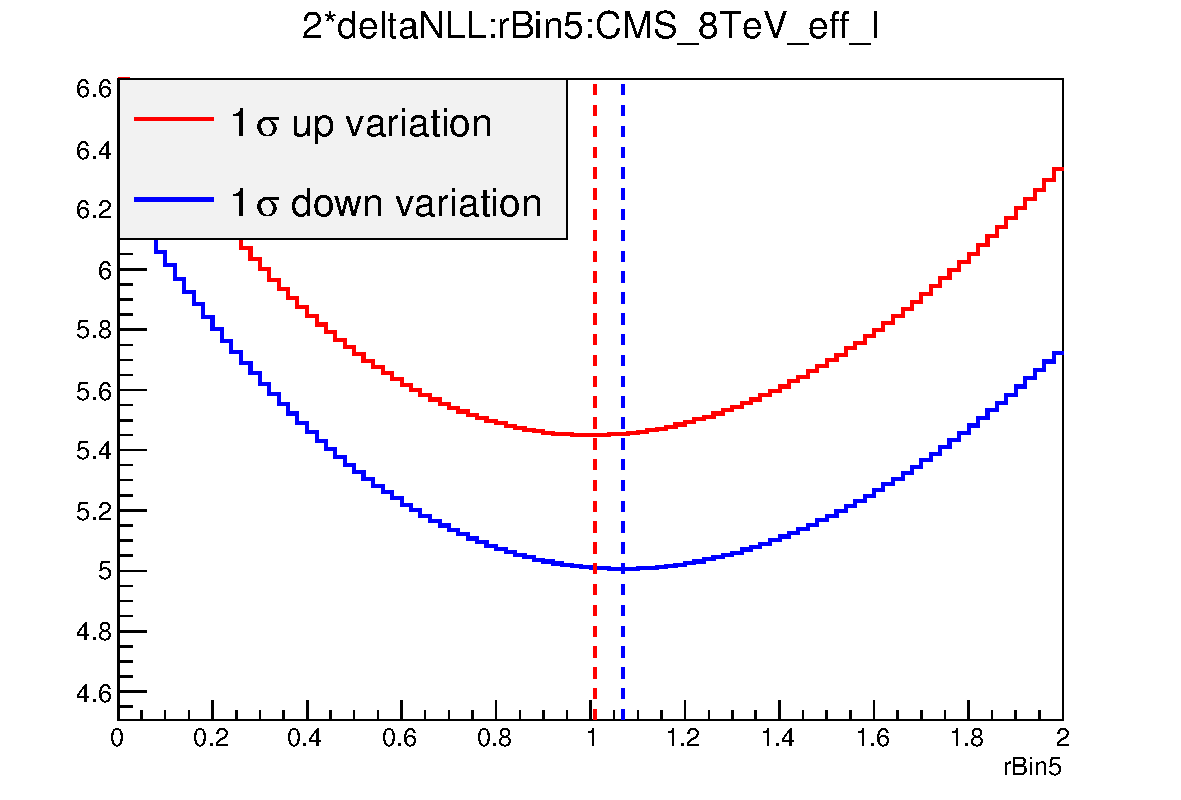
\includegraphics[width=0.45\textwidth]{images/bananas/profile_rBin5_CMS_8TeV_eff_l.pdf}}\\

\caption{{\bf Left side} Two-dimensional likelihood scan for lepton efficiency nuisance vs signal strengths in several bins: (a) bin 3, (c) bin 4, (e) bin 5. {\bf Right side} Likelihood profiles corresponding to the nuisance $\pm 1 \sigma$ up/down variations for (b) bin 3, (d) bin 4 and (f) bin 5.\label{fig:eff_l_bananas_p2}}
\end{figure}


\subsection{Type C errors}
Type C errors are those that only change the response matrix. They can be modeled with alternative response matrices that can be used to unfold the central fit result. A way to evaluate type C effects is the one depicted in Sec.~\ref{subsec:unfolding_closure}, i.e. either by taking an alternative model for \pth, or by varying the VBF/ggH ratio. It is important to note the either of those variations (JHU vs Powheg or variation of VBF/ggH) does not affect the shape of the signal templates, so it only affects the response matrix, and not the signal extraction.\\
We have checked that this is the case by comparing in shape the ggH and VBF templates in in each \pth bin. The comparison for \mll is shown in Fig.~\ref{fig:mlltemplatesseparate}. The differences are within the statistical accuracy of the samples.
\begin{figure}[tb]
\centering
\subfigure[]{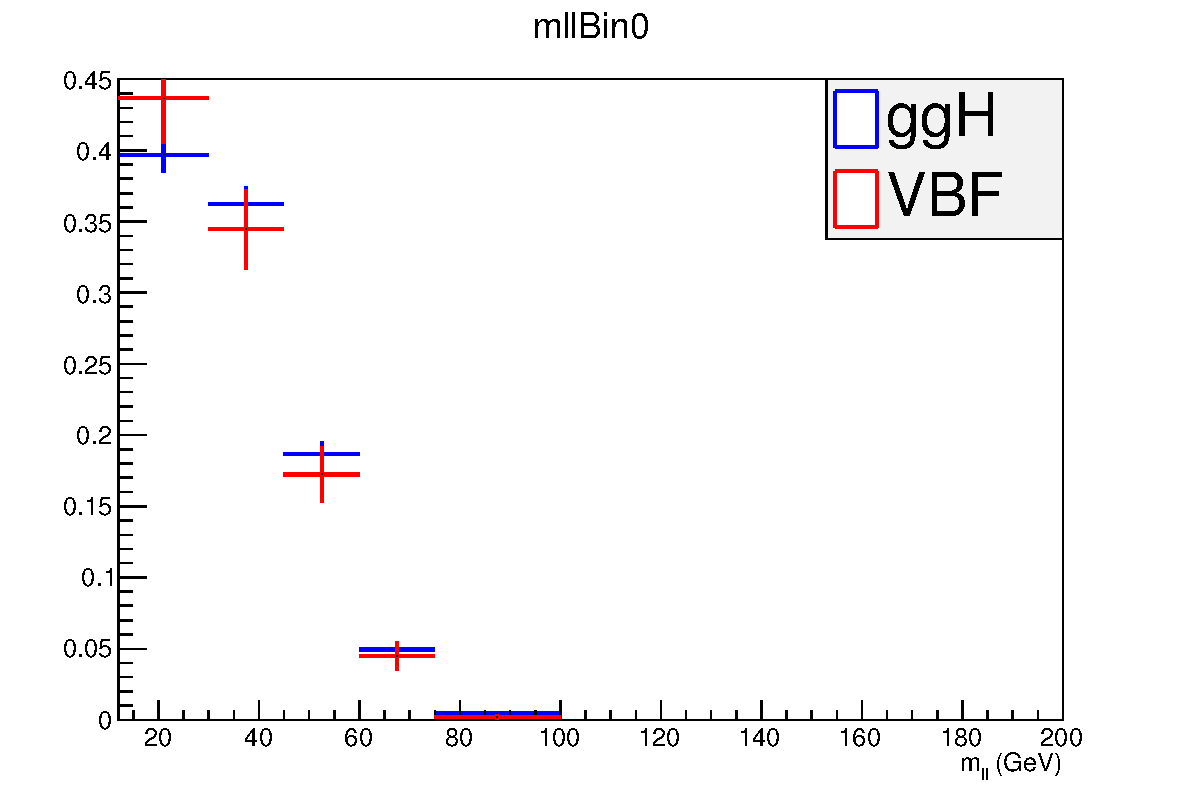
\includegraphics[width=0.4\textwidth]{images/HiggsShapesVBFggHComparison/mllBin0.pdf}}
\subfigure[]{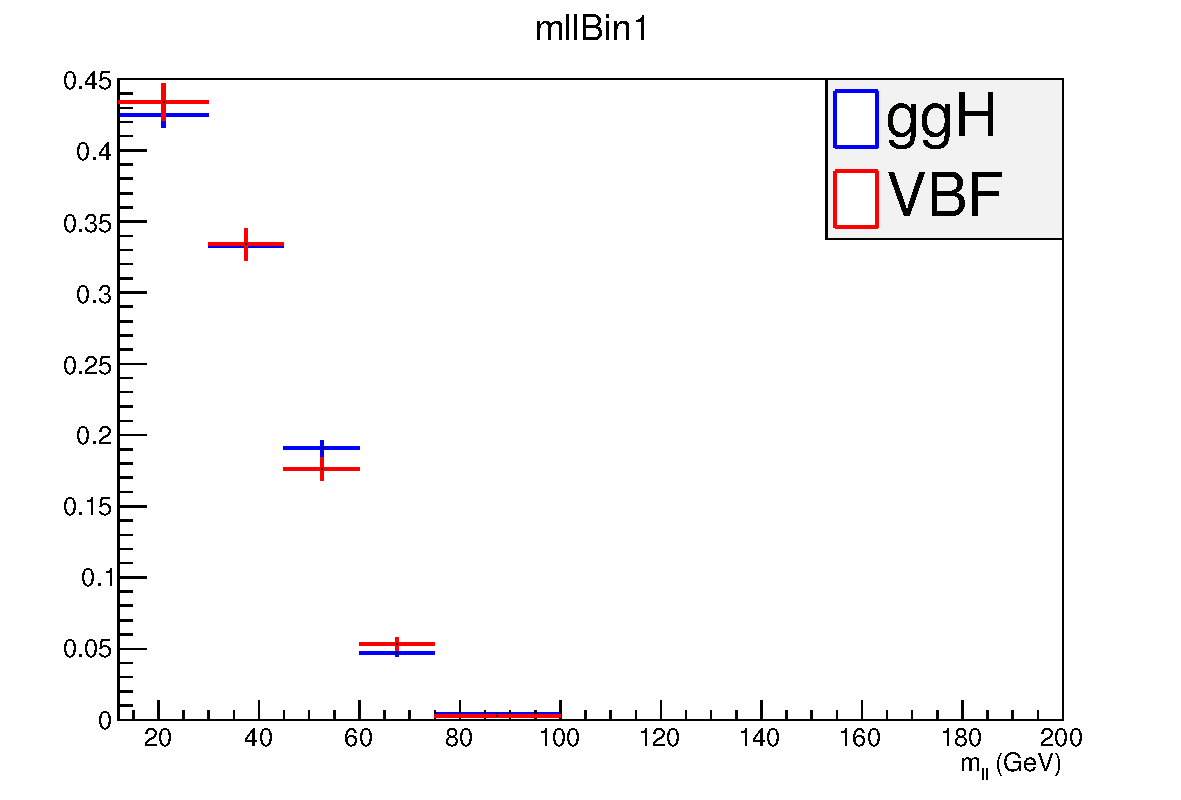
\includegraphics[width=0.4\textwidth]{images/HiggsShapesVBFggHComparison/mllBin1.pdf}}\\
\subfigure[]{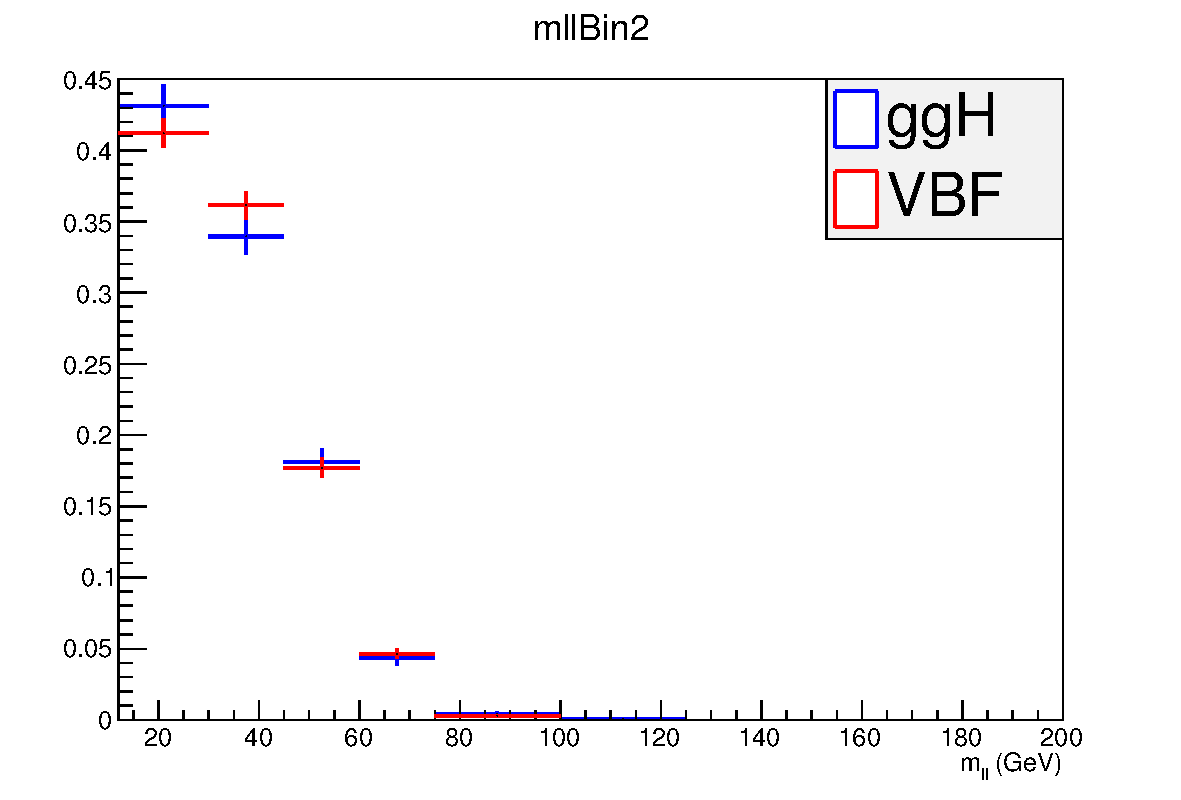
\includegraphics[width=0.4\textwidth]{images/HiggsShapesVBFggHComparison/mllBin2.pdf}}
\subfigure[]{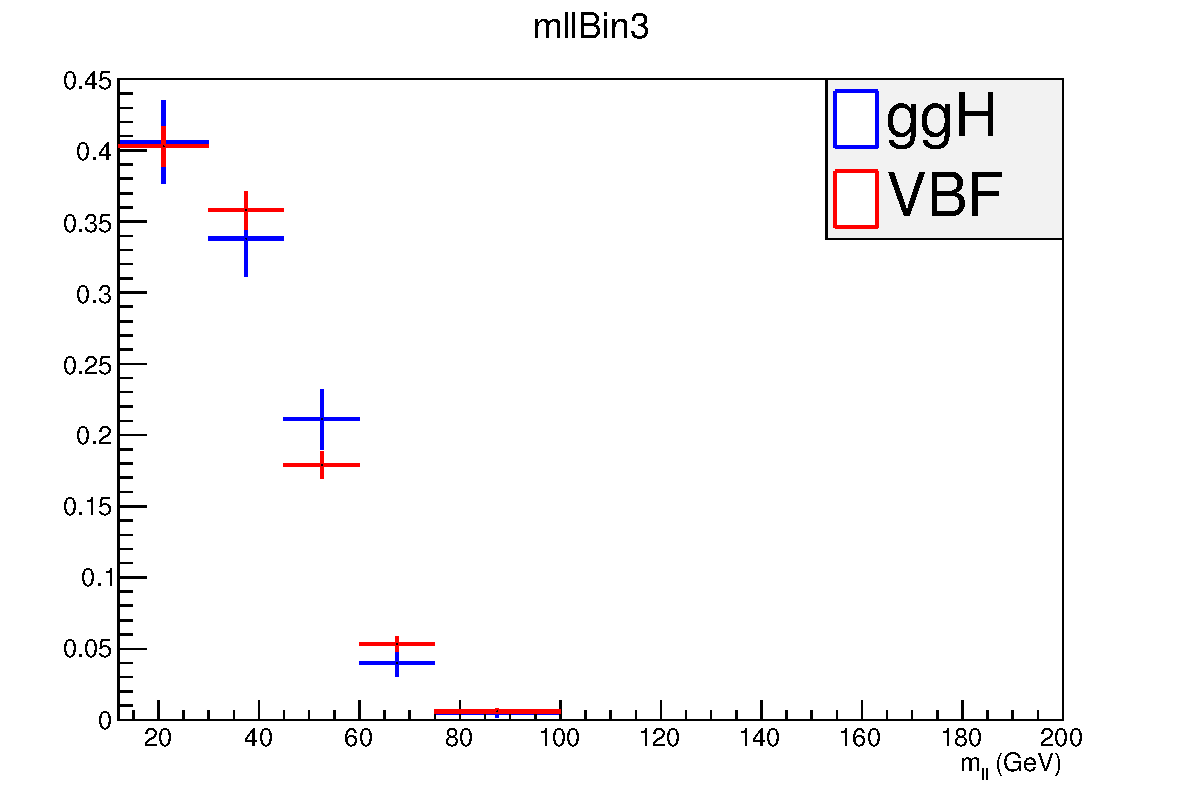
\includegraphics[width=0.4\textwidth]{images/HiggsShapesVBFggHComparison/mllBin3.pdf}}\\
\subfigure[]{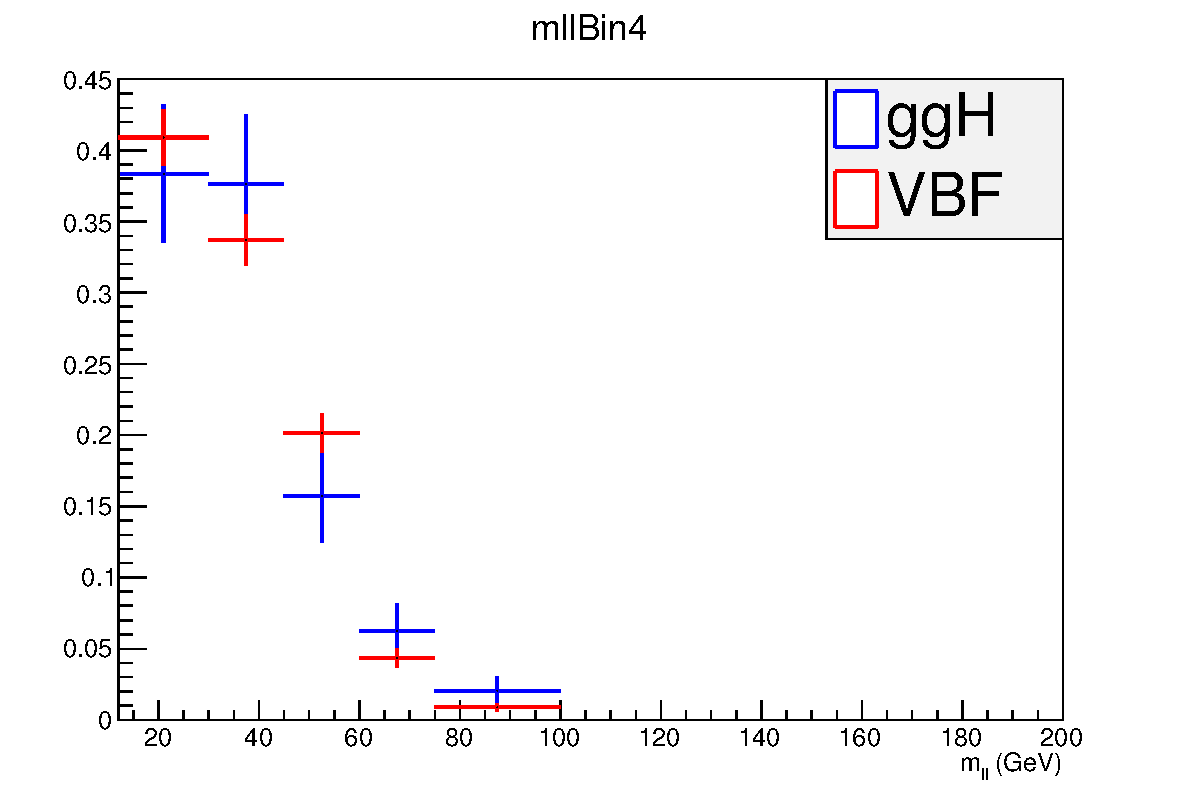
\includegraphics[width=0.4\textwidth]{images/HiggsShapesVBFggHComparison/mllBin4.pdf}}
\subfigure[]{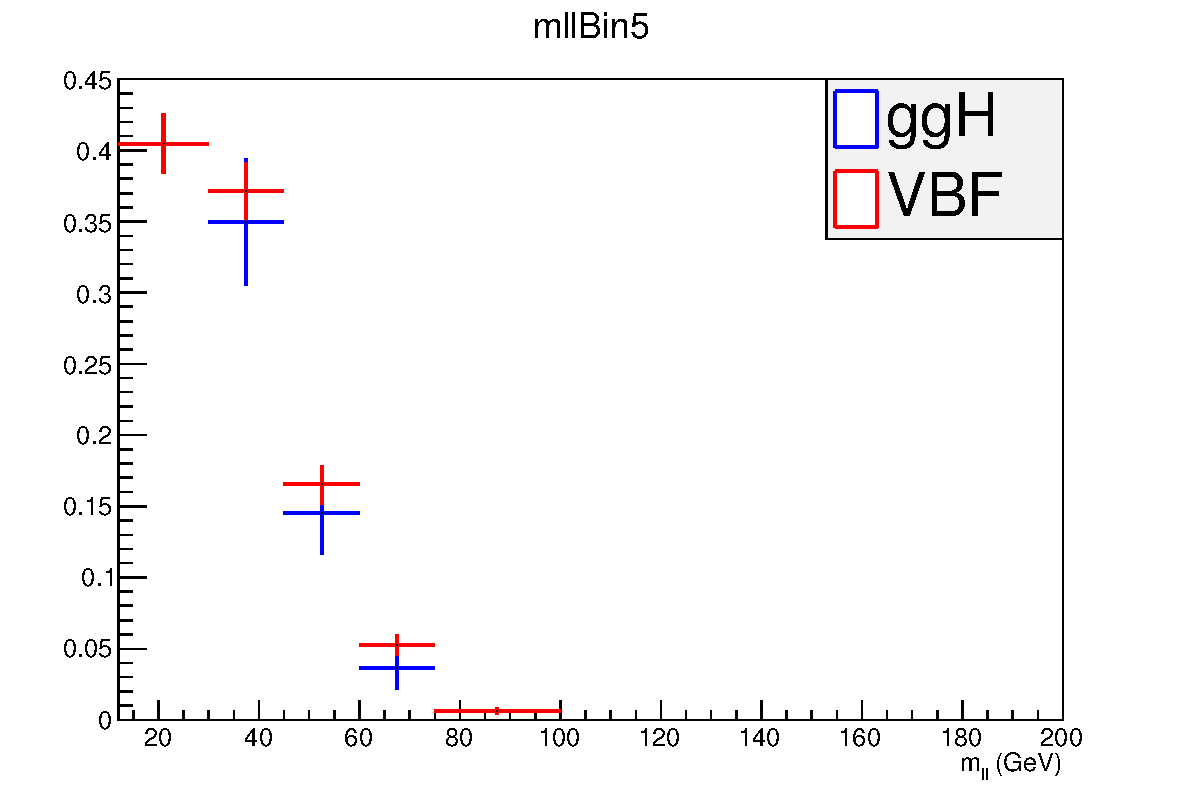
\includegraphics[width=0.4\textwidth]{images/HiggsShapesVBFggHComparison/mllBin5.pdf}}
\caption{Comparison of \mll template shapes in ggH and VBF samples.\label{fig:mlltemplatesseparate}}
\end{figure}

In order to assess whether the uncertainty on the VBF/ggH ratio has an effect on the signal extraction we have run three comparisons.
\begin{enumerate}
\item We have run 2000 MC toys for the full backgrounds+ggH+VBF expected spectra and we have fitted the signal yield in each bin both with the full ggH+VBF and with the ggH only template. The comparison is shown in Fig.~\ref{fig:templates_tests} (a).
\item We have run 2000 MC toys for the backgrounds+ggH spectra and we have fitted the signal yield in each bin both with the ggH only template and with the VBF only tamplate. The comparison is shown in Fig.~\ref{fig:templates_tests} (b).
\item We have run 2000 MC toys for the backgrounds+VBF (times 10) spectra and we have fitted the signal yield in each bin both with the VBF only template and with the ggH only tamplate. The comparison is shown in Fig.~\ref{fig:templates_tests} (c).
\end{enumerate}
\begin{figure}[tb]
\centering
\subfigure[]{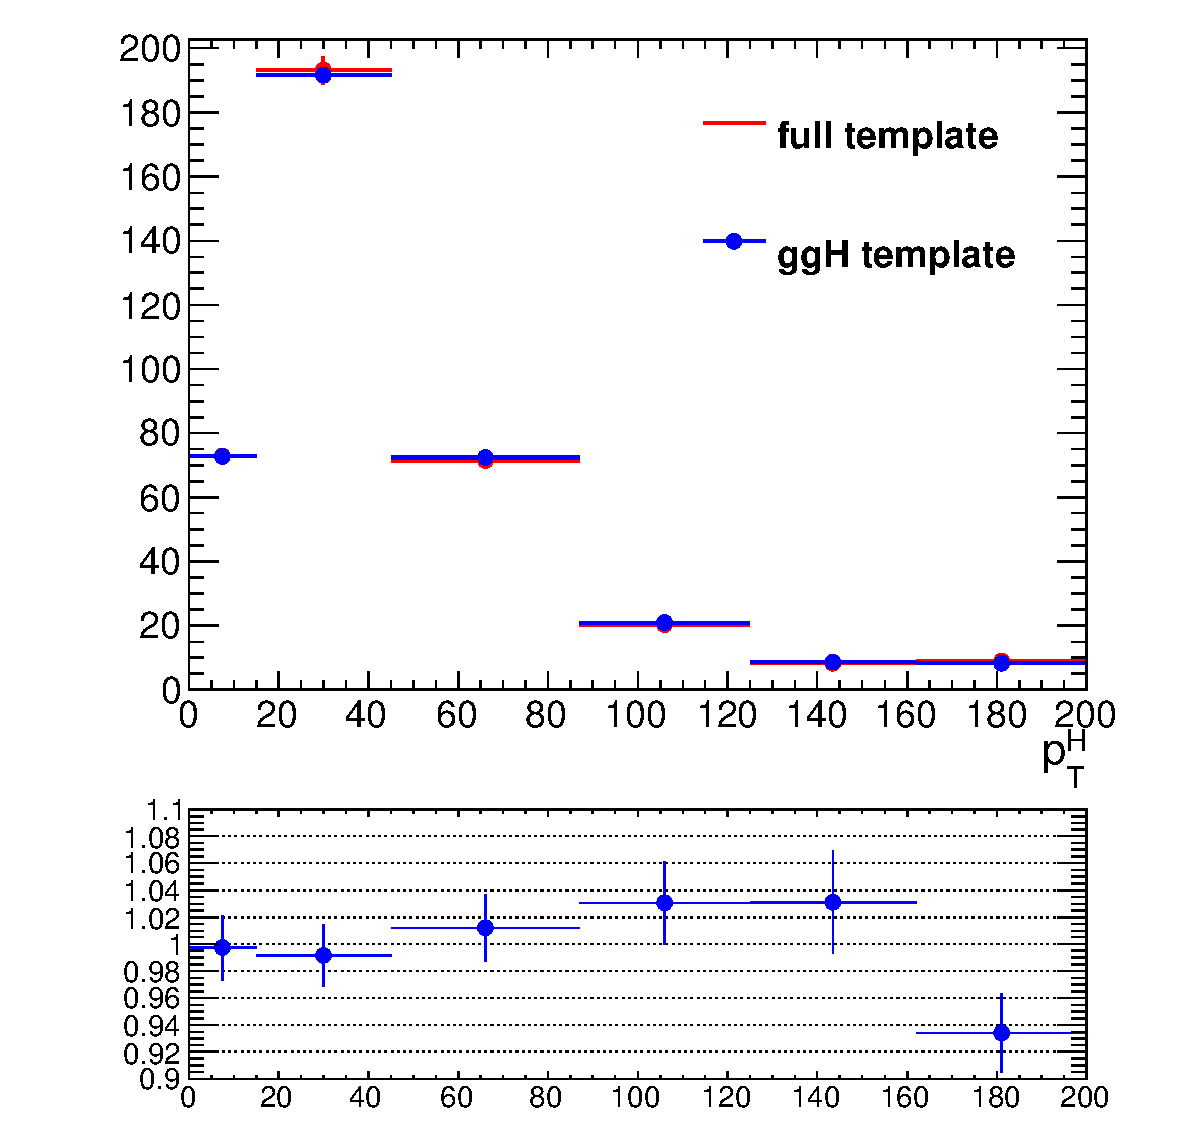
\includegraphics[width=0.4\textwidth]{images/gghTemplateOnFullToys.pdf}}\\
\subfigure[]{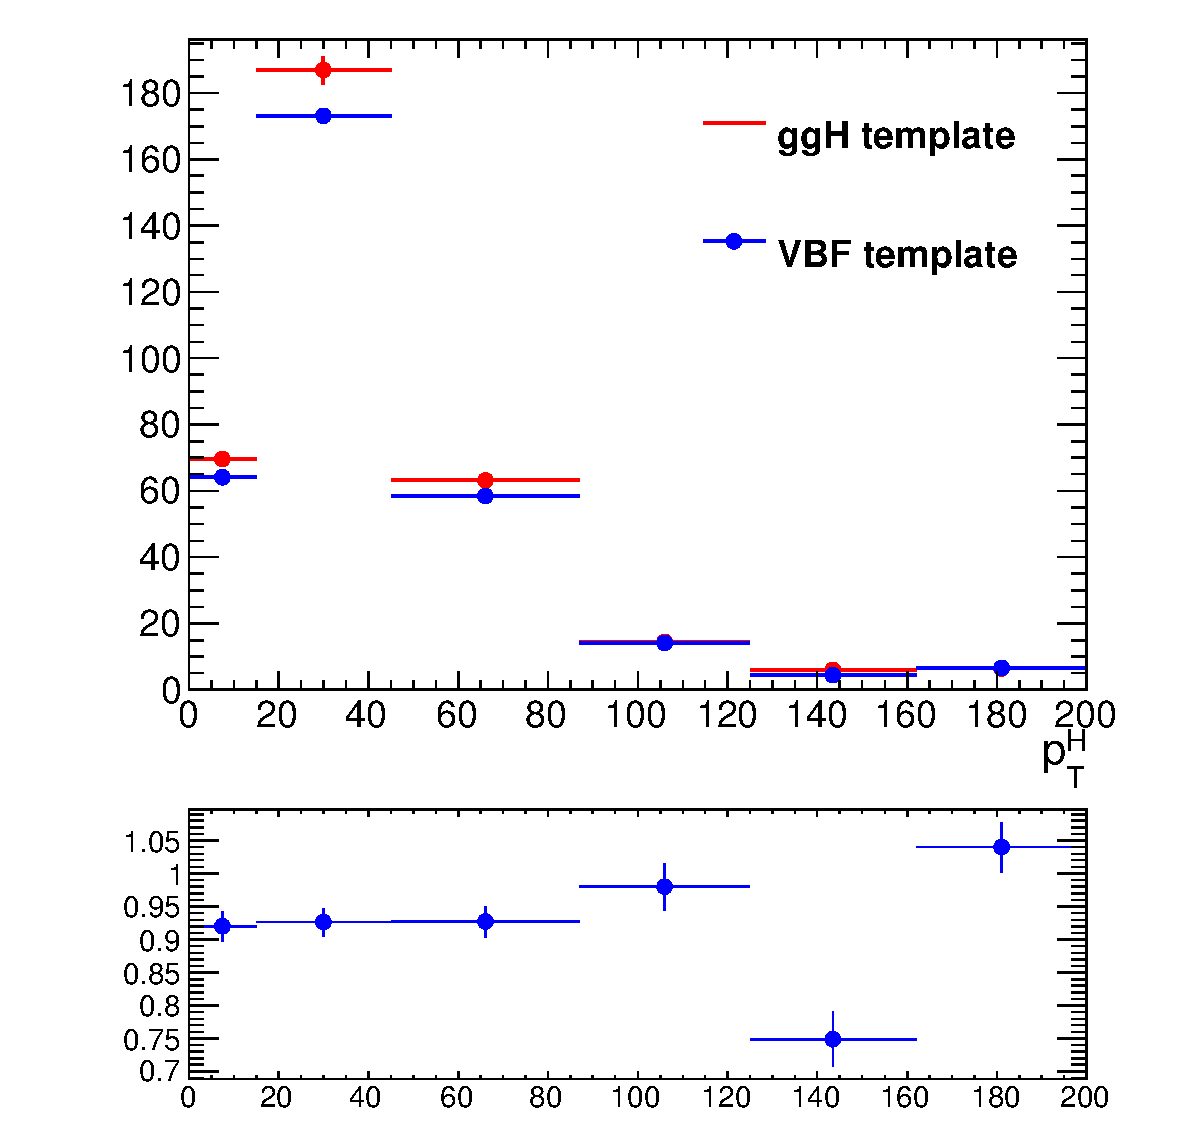
\includegraphics[width=0.4\textwidth]{images/VBFTemplateOnggHToys.pdf}}\\
\subfigure[]{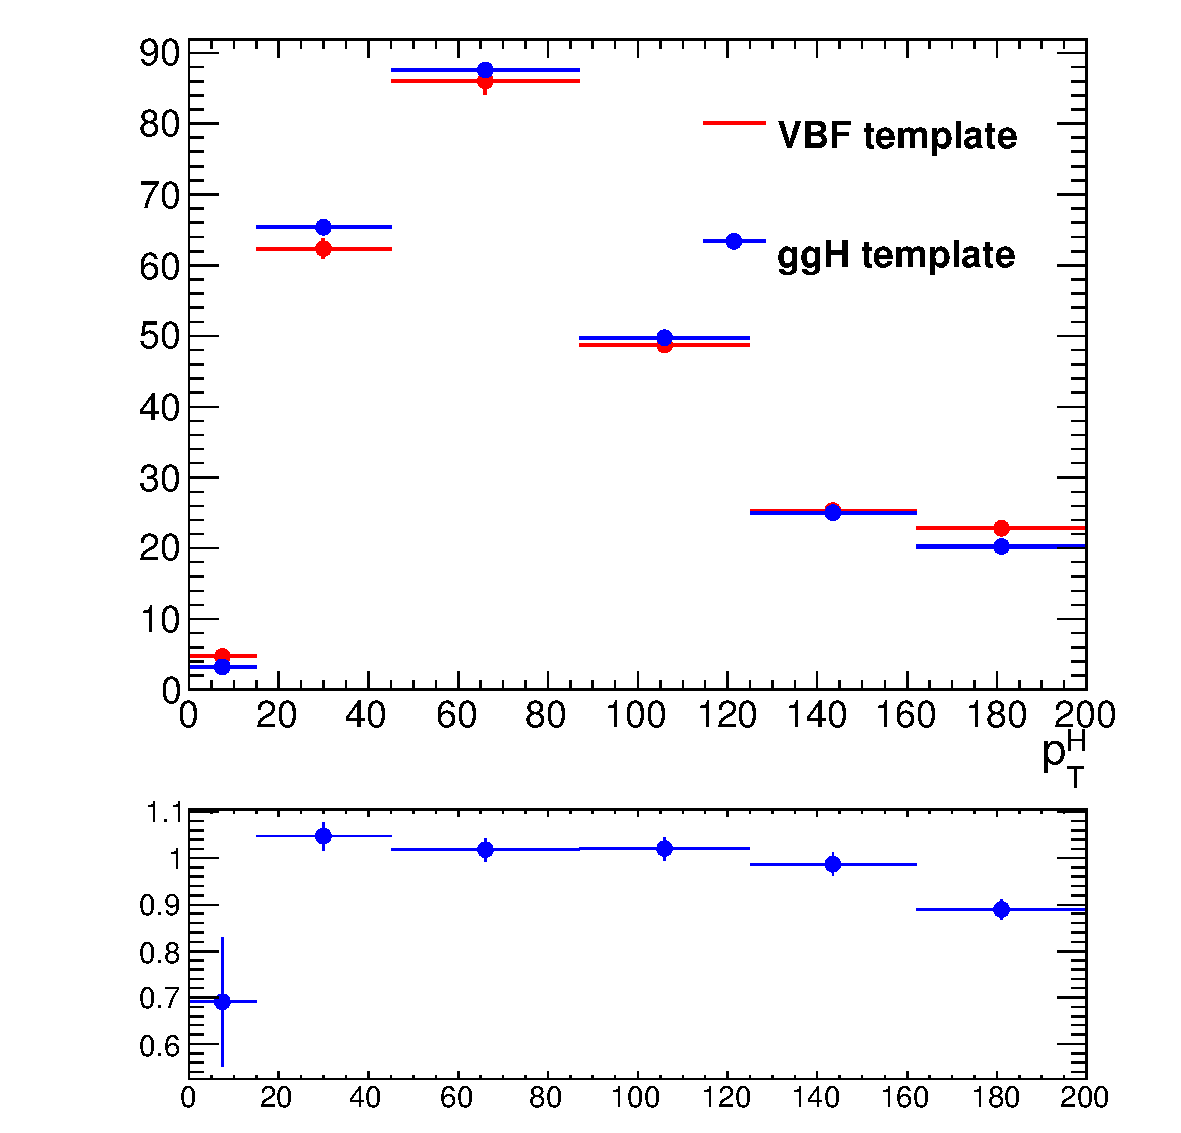
\includegraphics[width=0.4\textwidth]{images/ggHTemplateOnVBFToys.pdf}}\\
\caption{Signal yields extracted with different tamplates in the \mll-\mt plane. (a) average of 2000 toys produced with the full backgrounds+ggH+VBF template and fitted either with full ggH+VBF templates for \mll-\mt or with the ggH only \mll-\mt templates. (b) average of 2000 toys produced with the full backgrounds+ggH template and fitted either with ggH templates for \mll-\mt or with the VBF only \mll-\mt templates. (c) average of 2000 toys produced with the full backgrounds+VBF (times 10) template and fitted either with VBF templates for \mll-\mt or with the ggH only \mll-\mt templates. \label{fig:templates_tests}}
\end{figure}


%The effect of varying the VBF/ggH ratio is propagated through the unfolding and the corresponding uncertainty has been added together with the other type B uncertainties.
%The uncertainty coming from the JHU vs Powheg comparison are not taken into account but it is expected to be negligible.


\subsection{Combination of errors of different type}\label{subsec:embedded_unfolding}
In order to combine errors of type A, B and C after the unfolding we follow the following recipe: we sum in quadrature positive and negative errors separately, thus we obtain possibly asymmetric error bars. In case of type B errors that go in the same direction for both the up and the down variation, we propagate the maximum variation.


